% !TEX root = ../notes_template.tex
\chapter{Renal Clearance}\label{chp:blood_content}
Updated on \today
\minitoc

This chapter covers the concept of mass balance with a particular focus on water and electrolyte mass balance. The mass balance of water and electrolytes are supported by renal clearance which includes filtration, reabsorption and secretion for the formation and excretion of urine. Water and electrolyte mass balance are importance processes in the support of plasma (and therefore blood) volume; as well as the content and concentration of electrolytes in the extra-cellular fluid. In Chapter \ref{chp:ecf_microcirculation} it was clear that alterations in the plasma volume and concentration become transferred to the interstitial fluid and from there to the ICF. The regulation of body fluid volume and composition is accomplished by acting directly on the plasma. The kidneys, and other systems such as the gastrointestinal, metabolic, and pulmonary, participate in mass balance and the regulation of the body fluid volume and composition by acting on the plasma.

\vspace{5mm}

\textbf{Objectives include:}
\begin{enumerate}
    \item Explain mass balance.
    \item Relate mass balance to the ICF model and physical therapy practice. 
    \item Summarize the role of the kidneys.
    \item Explain the role of the kidneys in mass balance.
    \item Explain the functional anatomy of the kidney and nephron and the unique arteriole system including possible symptoms and signs of kidney conditions that should be part of the differential diagnosis of musculoskeletal back pain.
    \item Explain renal clearance.
    \item Explain urine formation and excretion by micturition.
    \item Explain the micturition reflex and the common cause of incontinence.
    \item Explain glomerular filtration, factors that influence GFR and the use of BUN and creatinine to assess GFR.
    \item Explain the role of tubular reabsorption and secretion and how they influence the excretion rate.
    \item Describe renal regulation of sodium, potassium, potassium, calcium, acid base balance.
    \item Explain renal regulation, and integration of, blood pressure, blood volume and osmolarity including the role of RAAS, angiotensin II, aldosterone and ADH.
    \item Explain the response to positive and negative water balance.
    \item Explain disturbances of osmolarity.
    \item Explain rhabdomyolysis and the possible role of water homeostasis on frailty in aging.
\end{enumerate}

\section{Mass Balance}

This chapter is the first to specifically discuss the concept of mass balance in clinical physiology. Mass balance applies the conservation of mass and energy to the analysis of physical systems. It considers the mass and energy entering (inputs) and leaving a system (outputs). Physical therapists help individuals maximize activity and participation such as activities of daily living (ADLs). ADLs are largely based on the need for water and nutrient input, and hygienic output of waste. To use the terms from the ICF model introduced in the Introduction, the inputs of food, drink and air require activity and participation (function). Many activities of daily living (ADLs) are based on the functional activities that provide appropriate inputs, and hygienic outputs required for physiological mass balance.

The inputs of food, drink and air ultimately provide the water, nutrients (macronutrients and micronutrients) and oxygen that are utilized for physiological processes. An overview of physiological mass balance is provided in Figure \ref{fig:mass_balance}. How these are used, whether they can be recycled, and the ways in which they are lost influences the time scale of the need for inputs. When describing outputs the term incidental loss refers to loss that occurs without purpose. Incidental loss is contrasted with intentional loss. Intentional loss is loss for a purpose, such as the loss of water in urine to regulate water balance. An example of incidental loss is the loss of $Ca^{2+}$ in the gastrointestinal tract due to sloughing of cells from the mucosal wall; and the loss of water with breathing.\footnotemark\footnotetext{It is interesting to consider whether losses such as $Na^+$ in sweat is incidental or intentional. It is clear that water loss in sweat is intentional - for the purpose of thermoregulation. While $Na^+$ loss is not needed for thermoregulation, its loss may help sustain ECF osmolarity. There are several additional examples that go beyond what we can consider here.}

% Consider the efficacy and integrity aspects of incidental losses.

%An example of incidental loss is the loss of $Na^+$ in sweat. The loss of water with sweat is purposeful as part of thermoregulation. But the loss of $Na^+$ with sweat is unnecessary for the primary purpose of thermoregulation, but still requires replacement of $Na^+$. Loss due to use such as oxygen in ETC, or due to a role being played in excretion of waste products such as water in feces and urine, is intentional loss. 

\begin{figure}[!h]
    \centering
    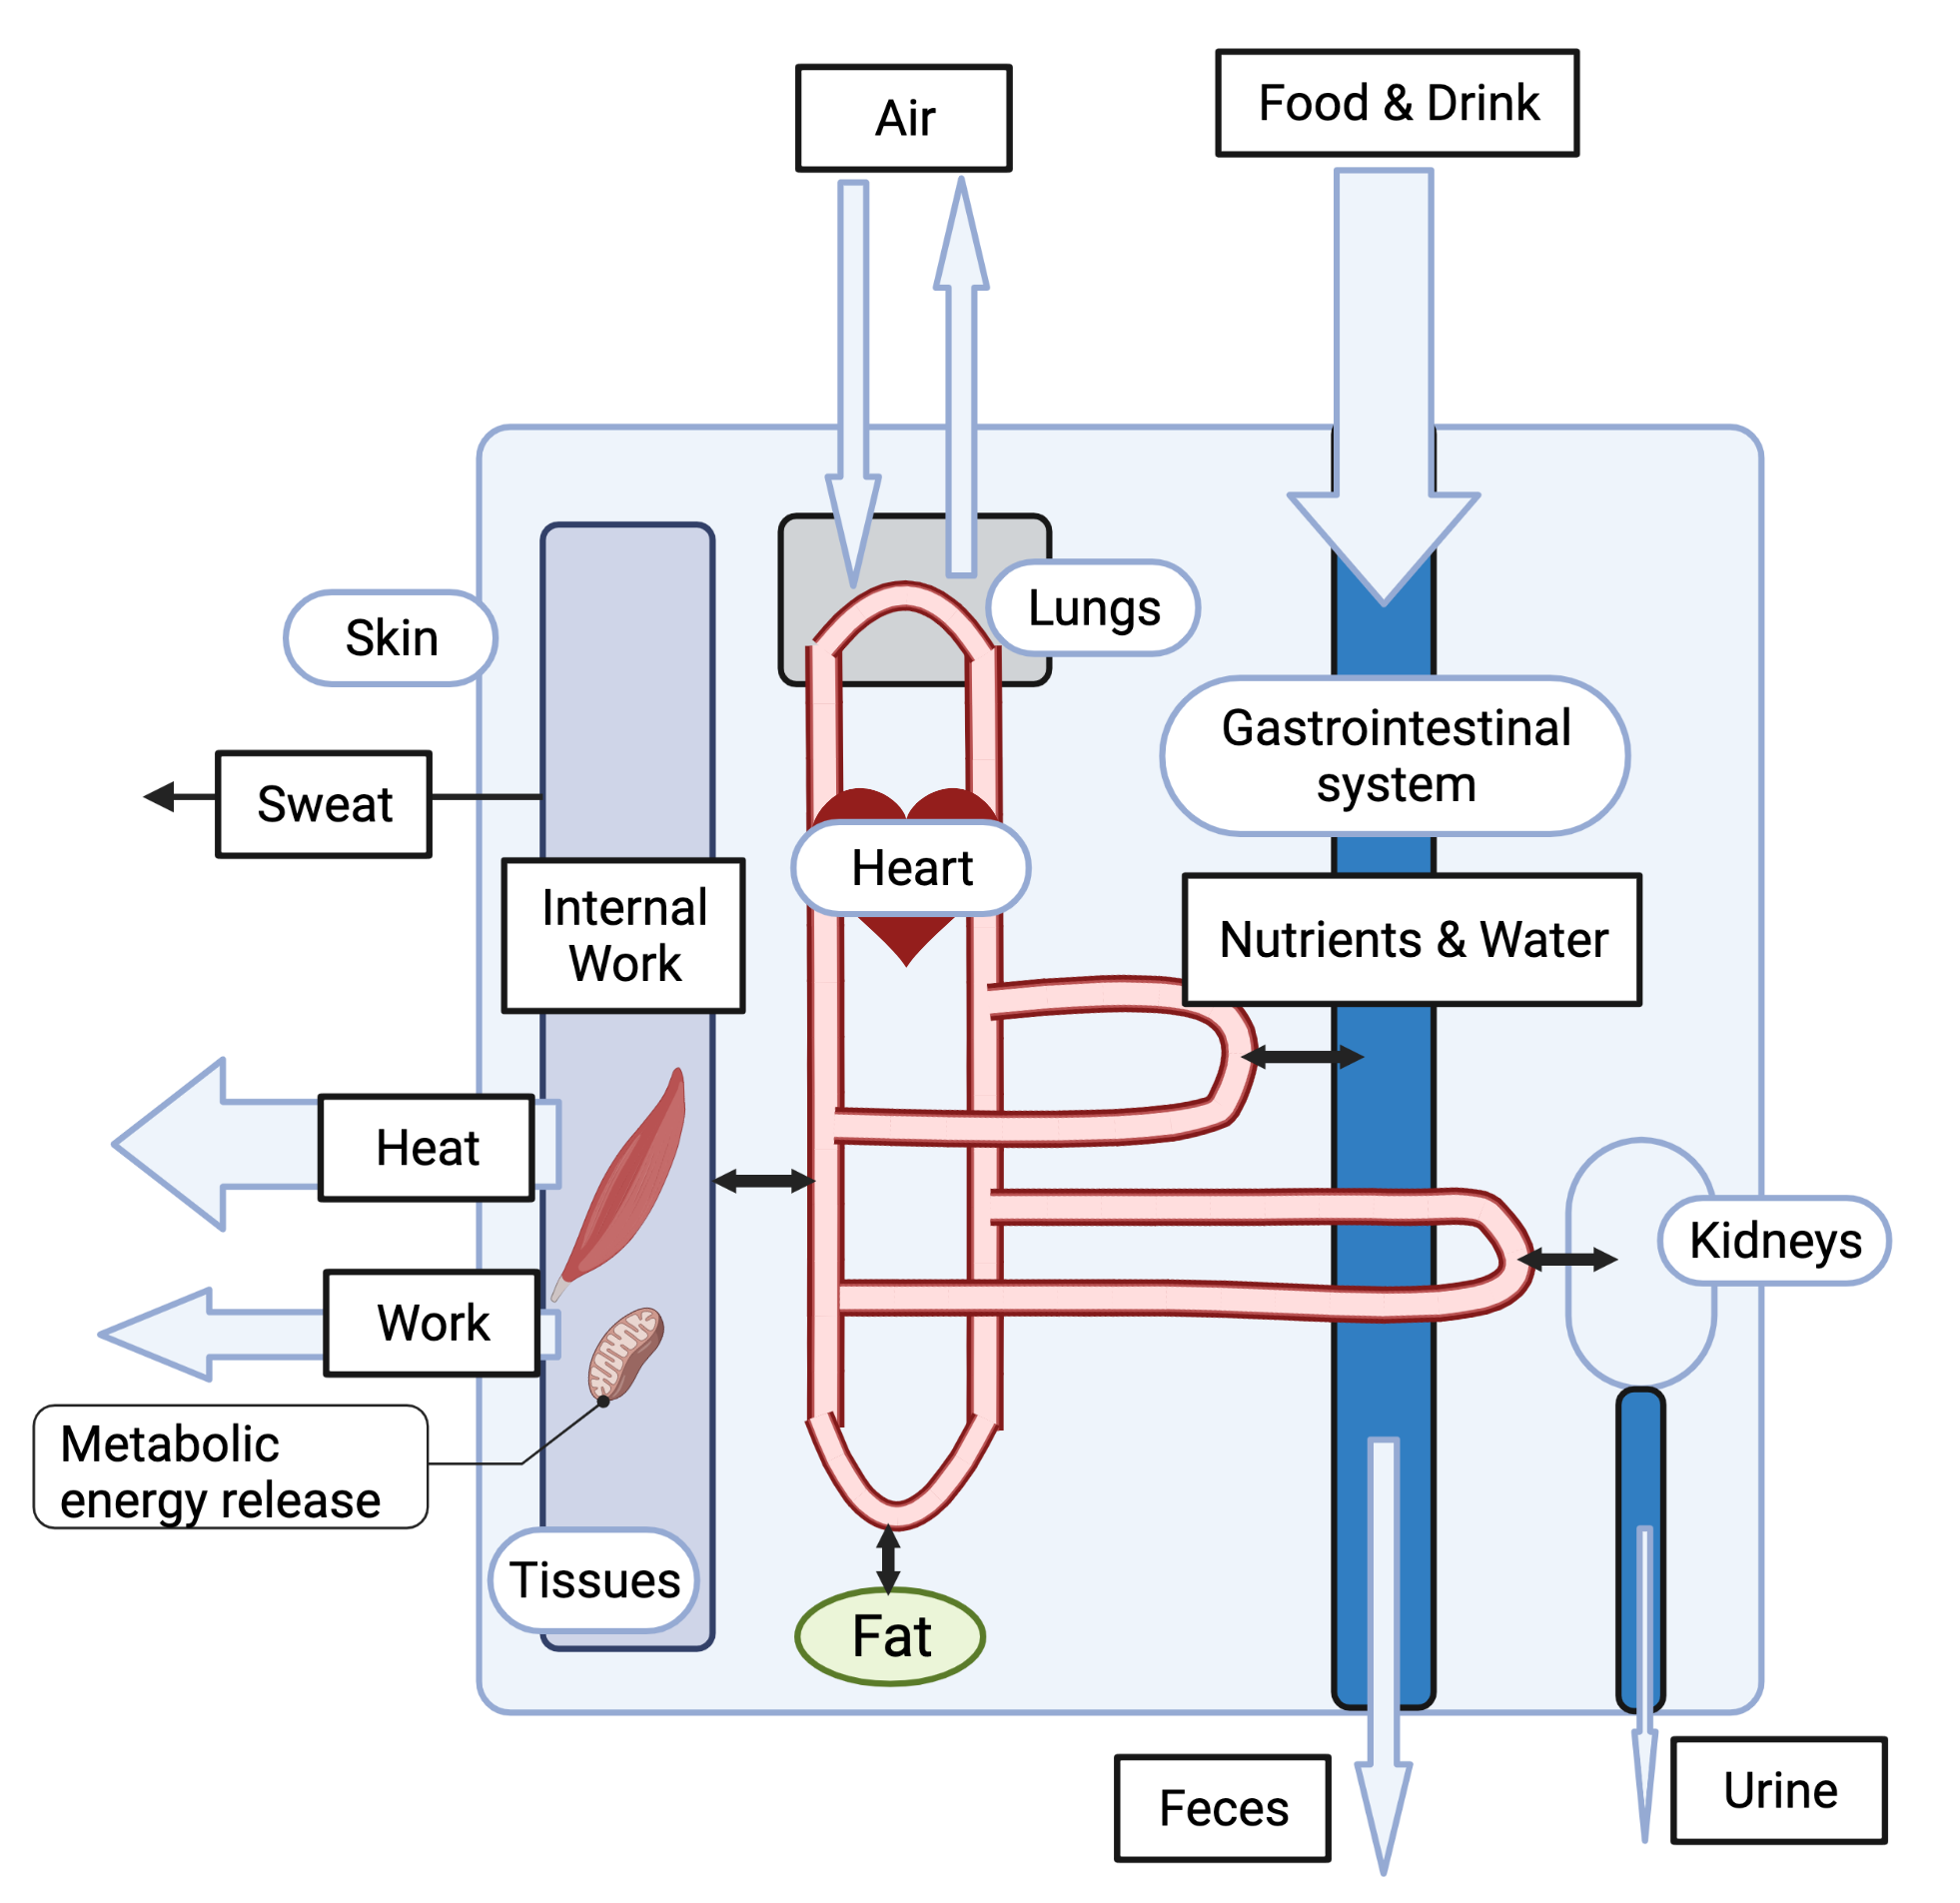
\includegraphics[width=1\linewidth]{./figure/mass_balance.png}
    \caption{Physiological Mass Balance \footnotesize{(Created with BioRender.com)}}
    \label{fig:mass_balance}
\end{figure}

\subsection{Oxygen Mass Balance}
Oxygen is used regularly and relatively quickly with very little storage (myoglobin) and no recycling, making the input of air with $O_2$ a regular requirement. Life is not sustainable for prolonged periods without the input of air with $O_2$ over the time scale of a few minutes in most individuals. At nearly the same rate, and at times at a slightly higher rate of oxygen utilization, carbon dioxide is produced as a waste product of mitochondrial respiration. Input and output of air allows for both the input of oxygen, and the output of carbon dioxide. Oxygen and carbon dioxide mass balance is covered in Chapters \ref{chp:blood_oxygen} and \ref{chp:alveolar_oxygen}.

\subsection{Nutrient Mass Balance}

When discussing mass balance of nutrients, which includes the consideration of diet and nutrition since it is about the input of nutrients, it is common to break nutrients into two main classifications. Macronutrients are larger molecules that can be utilized for energy purposes. They have an energetic, that is caloric, value in addition to other physiological roles they fulfill. Macronutrients include carbohydrate, fat and protein. Micronutrients are small molecules and in some cases simply elements or minerals. They do not have an energetic (caloric) value but are essential to many physiological processes. For muscle physiology it has already become clear that $Na^+$, $K^+$ and $Ca^{2+}$ are essential micronutrients. Up to this point micronutrients (dietary inputs) have been considered in their physiological roles. Electrolytes when considering the role they have in determining the osmolarity of a solution (e.g., $Na^+$); ions when considering the role they have in membrane potentials (e.g., $K^+$); and molecules when considering the role they play in activation (e.g., $Ca^{2+}$).

Macronutrients are routinely utilized for energy and system integrity (structural health of molecules such as hormones and neurotransmitters; as well as cellular structures, cells and tissues). However they are also stored purposely (fat is stored most abundantly as adipose tissue, carbohydrate as glycogen) or are available for extreme situations (protein is available for extreme situations from skeletal muscle). Proteins can be, at least partially, recycled. If a protein is broken down into amino acids and used to build an enzyme that is needed; it could be again broken down and used to build another enzyme. Similarly fat and carbohydrate utilized in structures can be recycled. However, macronutrients utilized for energy lose their structure and cannot be recycled, they must be replaced. The digestion of food to extract and absorb usable macronutrients\footnotemark\footnotetext{Once macronutrients are absorbed as carbohydrate or fat they are often referred to as substrates.} ultimately yields waste that remains in the gastrointestinal (GI) tract (for example, insoluble fiber) and is removed as feces. 

The lining of the GI tract not only absorbs all nutrients (macro and micro), but there is some incidental loss of micro-nutrients (electrolytes and minerals) such as $Ca^{2+}$ in the feces from the GI secretions and normal wear and tear of the cells and tissue that line the GI tract. A small amount of incidental loss of micronutrients such as $Na^+$ and $K^+$ occurs in the sweat and urine. Since the input of input of these micronutrients can easily exceed the incidental loss, there can be intentional (regulated) loss through the renal filtration, reabsorption and secretion processes to maintain $Na^+$, $K^+$ and $Ca^{2+}$ homeostasis.

Macronutrient mass balance is covered in Chapter \ref{chp:blood_nutrients} on Digestion, Absorption and Metabolism.

\subsection{Water Mass Balance}

Water is the source of the fluid environment that the biochemical processes of life occur, and transport of essential nutrients flow through the circulation and micro-circulation. Without water the blood plasma, interstitial fluid and intra-cellular fluid would not be fluid. The fact that they are fluid enables nutrient movement. The amount of water in the body also influences the concentration (and therefore osmolarity) of these fluid spaces. The amount of water influences the blood volume. If blood volume is too high, blood pressure increases and edema may result. If blood volume is too low, viscosity increases which increases resistance to circulation. Problems occur when there is too little water (dehydration) or too much water (elevated blood volume, edema). The water in the body is always in use, being filtered between compartments in support of the movement of nutrients and electrolytes as well as by-products (waste). In this way it is recycled - there is no need for a complete overturn of water in the course of a day. However, the amount of water that must be taken in (input) should equal the amount of water that is lost in a day (output). Water loss occurs through four routes, two incidental and two intentional. Incidental water loss occurs with ventilation of air out of the body; and a small amount of water is routinely lost in the feces (it could be argued that water loss with feces (stool) is intentional to avoid hard difficult to pass stool. Evaporation of water from the skin is a mechanism of cooling the body and sweating is a route of loss. Intentional loss of water in sweat is highly variable based on the temperature and activity levels which influence the need for cooling. Renal filtration and excretion requires a loss of water in urine for the removal of metabolic waste. Of these four routes for the output of water sweating is highly variable and can be partially regulated through behavioral adaptations; renal is also highly variable and is regulated through physiological processes. The maintenance of normal water volume, and as a result plasma volume, is buffered by fluctuations in renal output in response to water input. Because there is a continual regular loss of water (breathing and sweating), and a necessary regular loss of water for waste removal (feces and urine), there is a regular need (demand) for water input. While the kidneys can make more or less concentrated urine which includes less or more water (respectively), the body must make urine regularly to filter the blood and keep it free from the toxicity of metabolic waste products.

\subsubsection{Blood Volume Composition}

Blood volume includes plasma (approximately 55\%) and cells (See Figure \ref{fig:Hematocrit}). Most of the plasma is water. Most of the cells are red blood cells (RBCs) and are also called erythrocytes. RBCs contain hemoglobin (HgB). RBCs are the oxygen carrying cells in blood and are discussed more thoroughly in Chapter \ref{chp:blood_oxygen} on Respiration. The measure referred to as hematocrit (HcT) reports on the percentage of blood that contains RBCs. Since other cells occur in relatively low volume, it is acceptable to consider plasma as simply 1 minus HcT when HcT is reported as a fraction (HcT of 45\% is 0.45). If HcT is 0.45, then 1-0.45 = 0.55, which means 55\% of the blood is plasma.

\begin{figure}[!h]
    \centering
    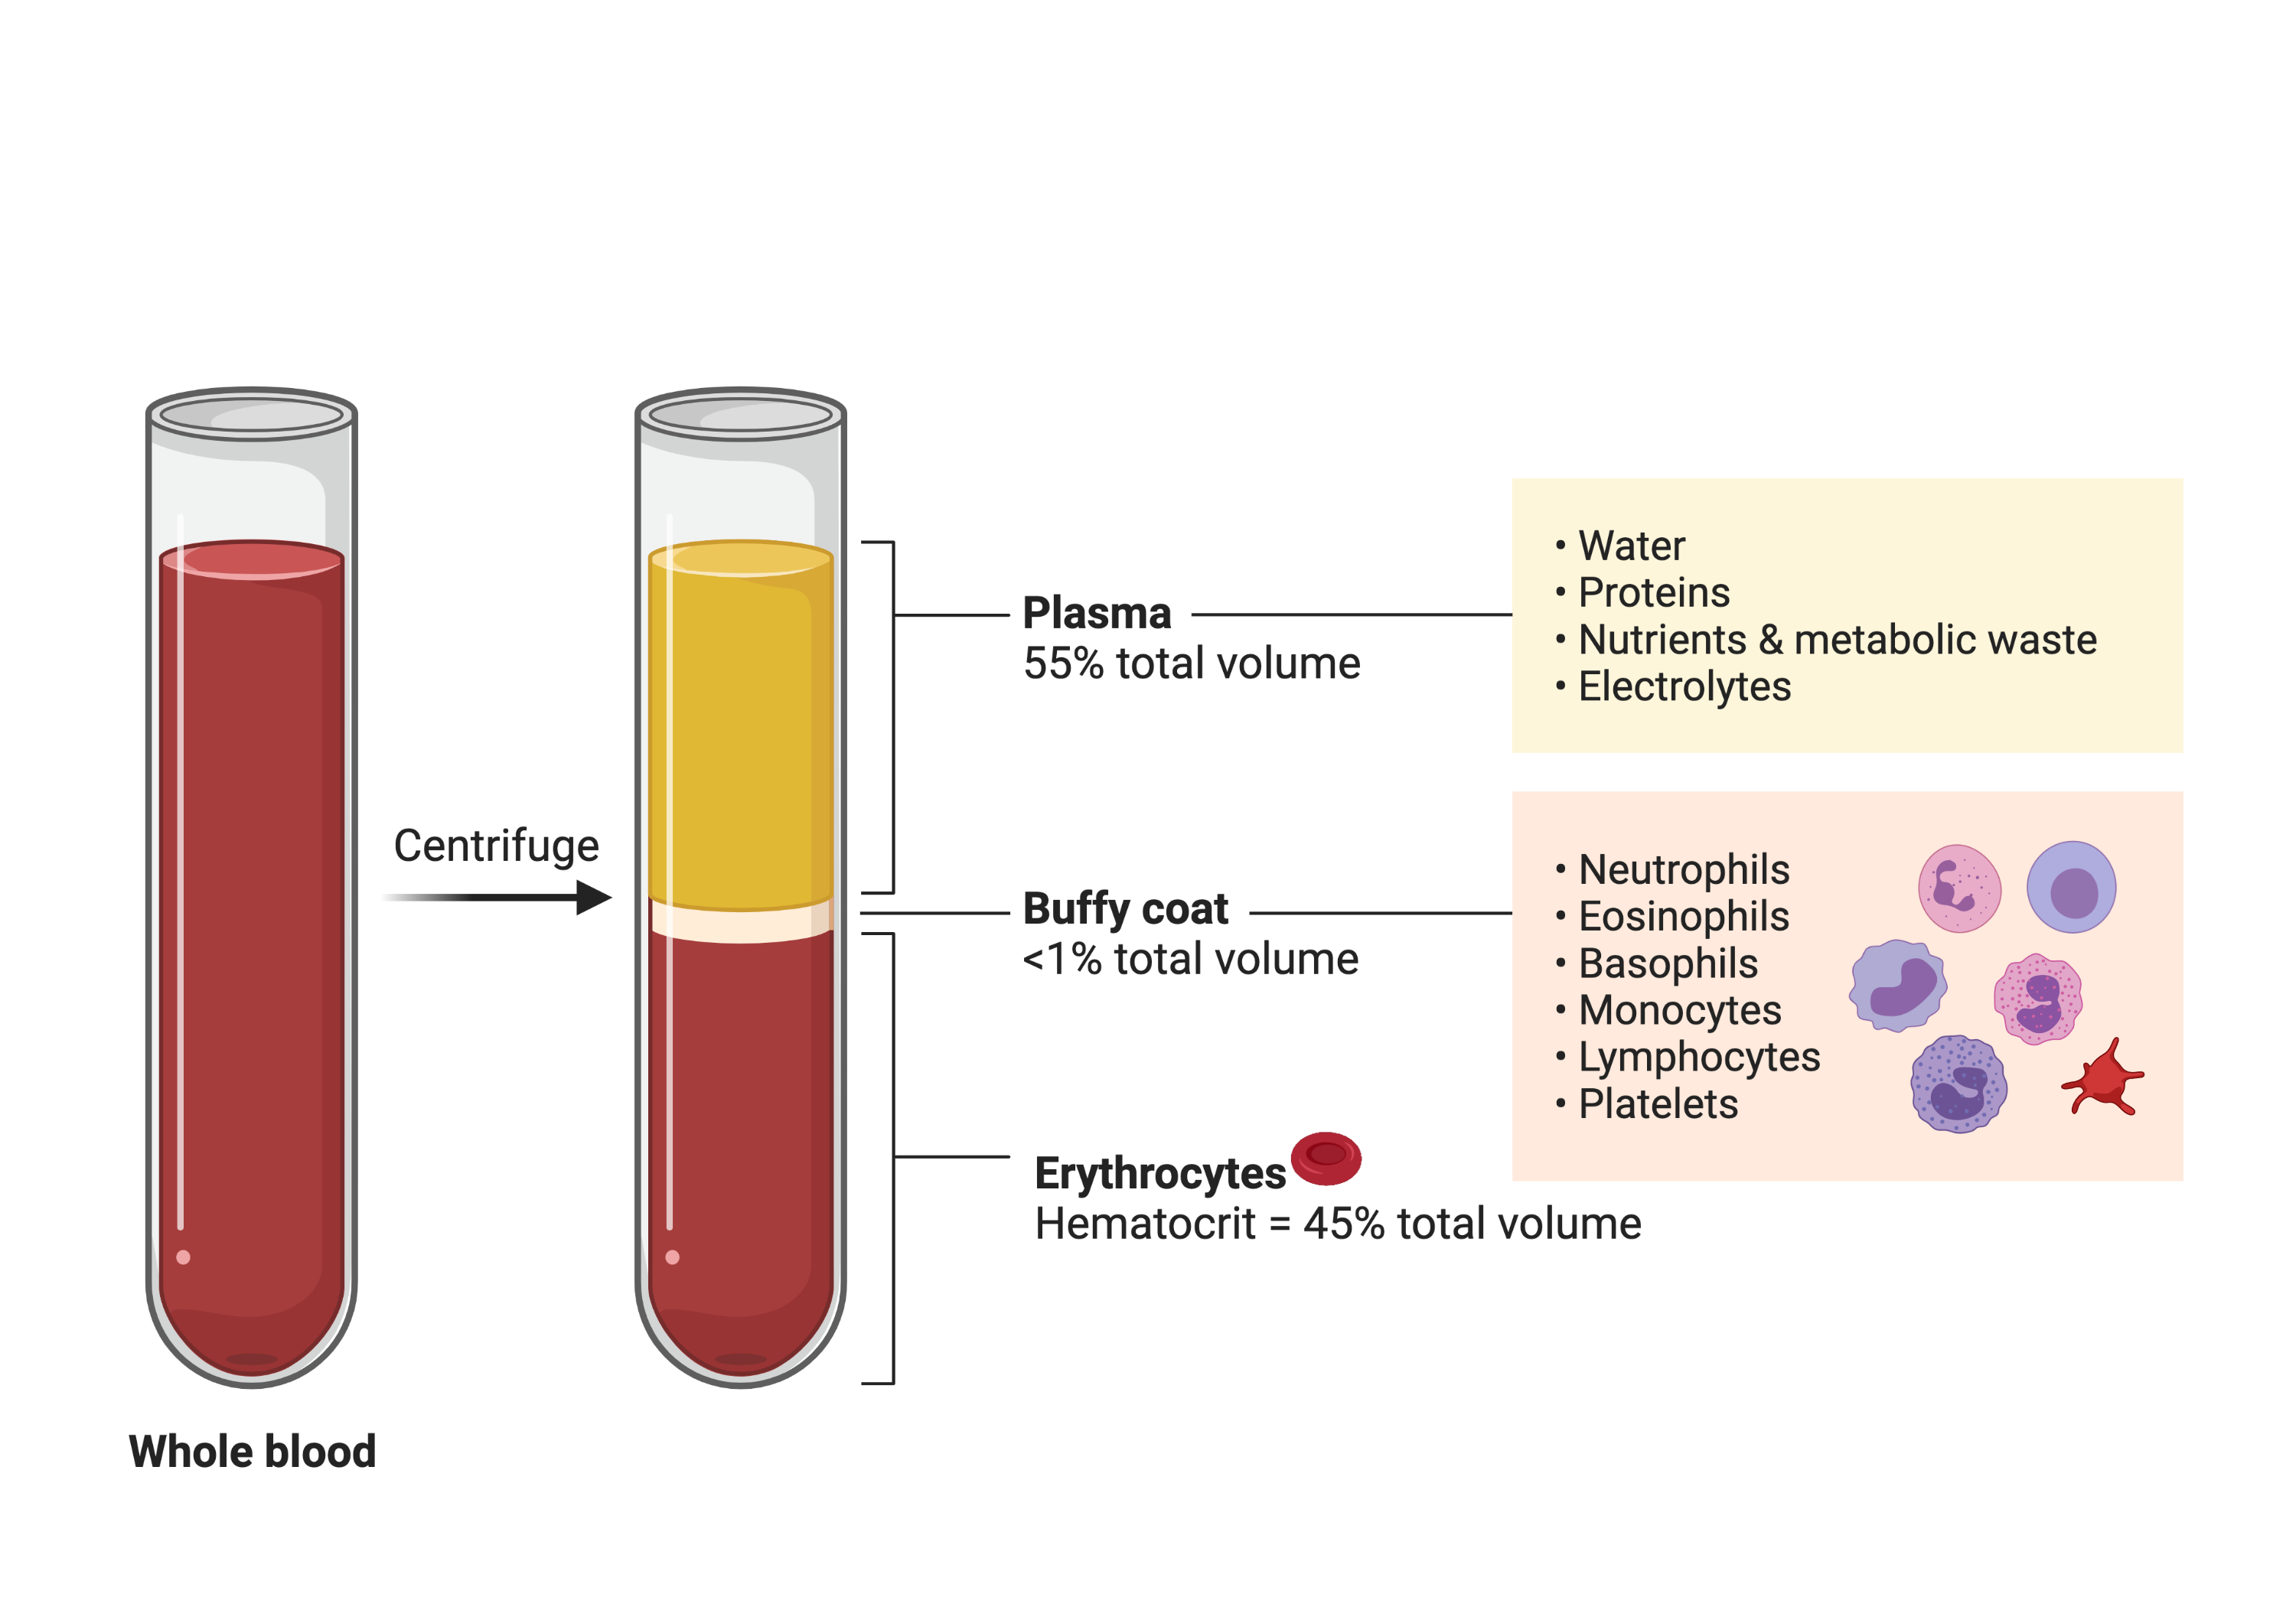
\includegraphics[width=1\linewidth]{./figure/Hematocrit.png}
    \caption{Plasma \& Hematocrit of Blood \footnotesize{(Created with BioRender.com)}}
    \label{fig:Hematocrit}
\end{figure}

\section{Renal Function}

Renal function relies on the kidneys. The kidneys have several important physiological functions summarized below and in Figure \ref{fig:Renal_Functions}. 

\begin{enumerate}
    \item Excretion: The kidneys ensure that harmful substances are excreted in urine. Harmful substances can be absolutely harmful (waste products such as urea and creatinine), or relatively harmful (electrolytes when they exceed their normal ranges).
    \item Regulation \& Buffer by Excretion: The kidneys regulate and therefore buffer the mass balance of plasma, and therefore body water and electrolyte amounts. Through both water and the electrolyte content they regulate electrolyte concentration.
    \item Regulation by Excretion: Through the regulation of plasma volume the kidneys provide long term regulation to blood pressure.
    \item Regulation by Hormone Secretion: The kidneys synthesize and secrete three hormones:
    \begin{enumerate}
        \item Renin for the regulation of blood pressure
        \item Erythropoietin for the regulation of red blood cells
        \item 1,25-dihydroxycholecalciferol for the regulation of $Ca^{2+}$
    \end{enumerate}
\end{enumerate}

Functions 1, 2 and 3 and the endocrine function of renin are covered in this chapter. The endocrine function of erythropoietin is covered in the Chapter \ref{chp:blood_oxygen} on Respiration; and of 1,25-dihydroxycholecalciferol in Chapter \ref{chp:blood_nutrients} on Digestion-Absorption-Metabolism.

Functions 1 and 2 are accomplished through renal clearance. Renal clearance is a general concept that describes the rate that substances (including water) are removed from plasma. Renal clearance is accomplished as blood passes through the renal capillaries and undergoes ultrafiltration. The ultrafiltrate proceeds through the renal tubule while the more selective processes of reabsorption and secretion fine tune the content of urine for clearance. In total, renal clearance ensures that harmful substances are excreted (filtered and not reabsorbed); that the correct volume of water and electrolytes remain in the plasma (filtered and then reabsorbed as necessary, or not filtered and secreted as necessary). 

\begin{figure}[!h]
    \centering
    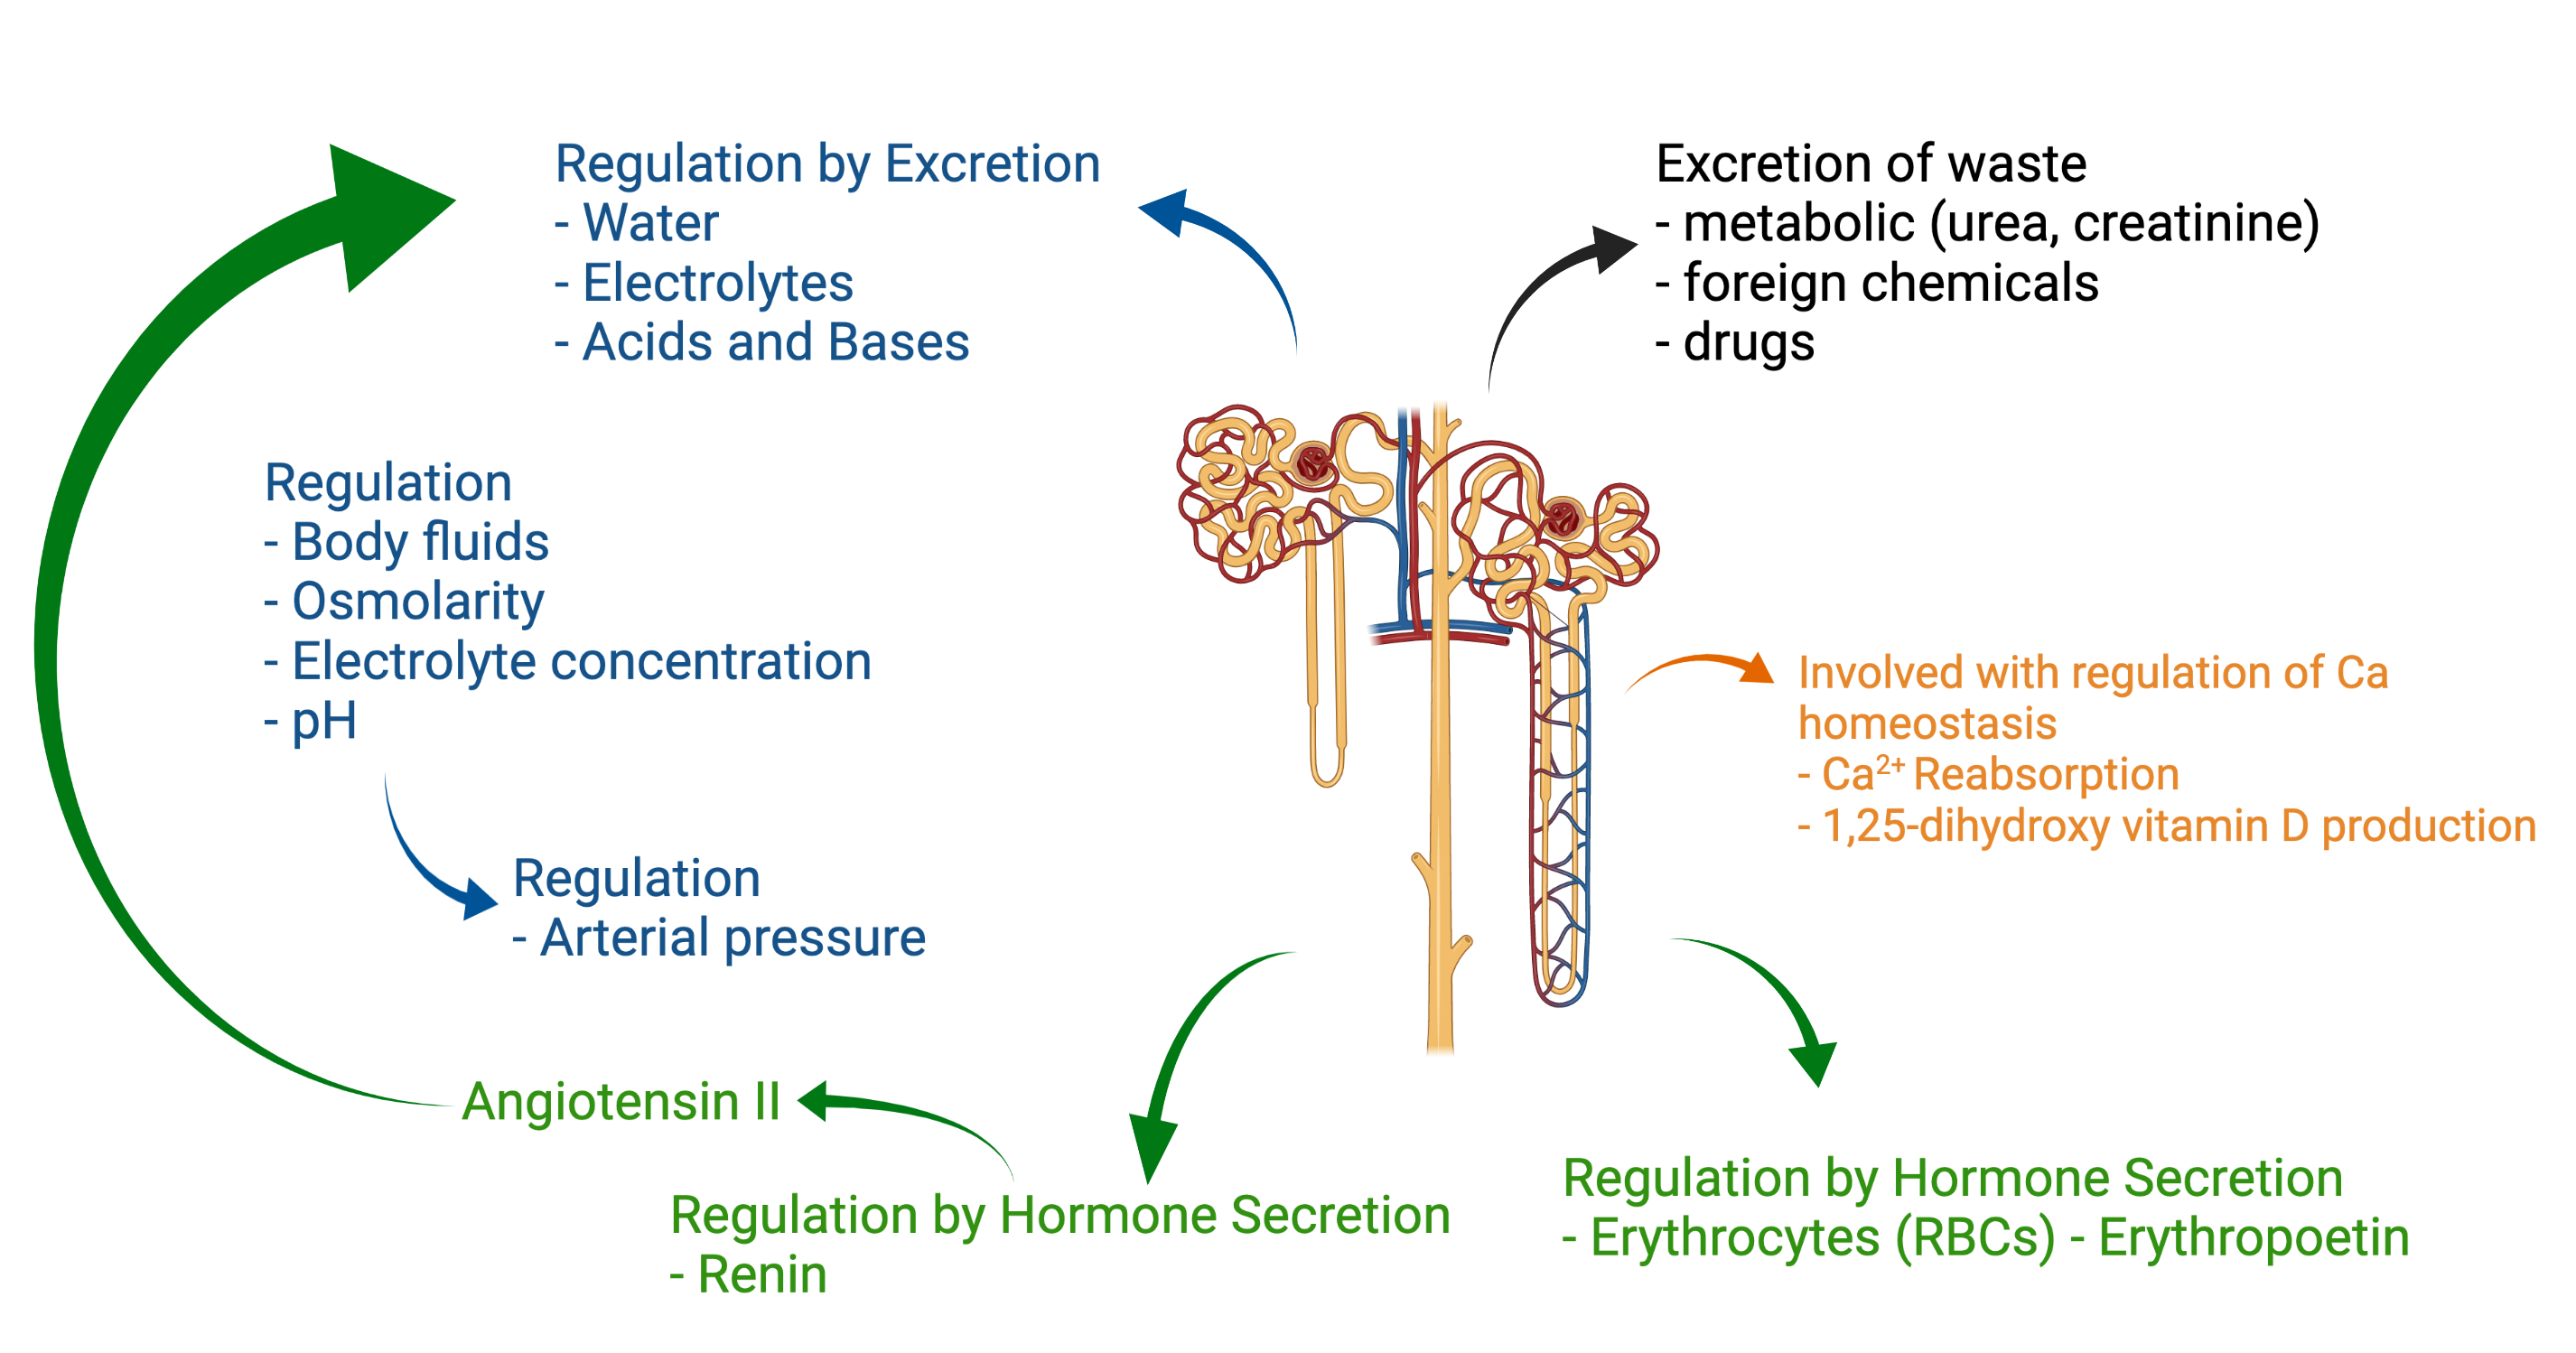
\includegraphics[width=1.0\linewidth]{./figure/Renal_Functions.png}
    \caption{Overview of Renal Functions \footnotesize{(Created with BioRender.com)}}
    \label{fig:Renal_Functions}
\end{figure}

\subsection{Functional Anatomy}

The kidneys are in the retroperitoneal cavity of the body.  Given their location and the high prevalence of back pain in physical therapy practice it is important to consider the possibility that back pain is related to the kidneys. Kidney pain is pain from disease or injury to a kidney. Kidney pain or discomfort may manifest as a dull, one-sided ache in the upper abdomen, side or back. Back pain that includes upper abdomen or side components and that does not respond to provocations that would typically provoke a musculoskeletal source of pain such as movements (active \& passive tension) should be considered. The patient should be questioned regarding a history of the common causes of kidney diseases such as alcohol use, diabetes, high blood pressure, family history or a history of kidney stones. Fever and changes in urinary habits or urinary symptoms often accompany kidney pain and are therefore important considerations when ruling out a kidney as a source of back pain.

%Need some examples of pathology of visceral vs. MSK origin

Each kidney is divided into two regions: the outer cortex and the inner medulla. Comprising these two region are tube-like structure called nephrons - the functional unit of the kidney. Each kidney can contain approximately 1 million individual nephrons with each nephron serving a vital role in reabsorption, secretion, and filtration of solutes. At its simplest, each nephron contains a renal corpuscle (glomerulus surrounded by Bowman’s Capusle) and renal tubule. The glomerulus is a capillary network and the primary site for plasma filtration and the formation of urine. Distributed on both ends of the glomerulus are the afferent and efferent arterioles, which provide inflow of filtrates to the glomerulus and outflow of filtrates to the upper portion of the nephron - the Bowman’s Capule (or Bowman’s Space).

\begin{figure}[!h]
    \centering
    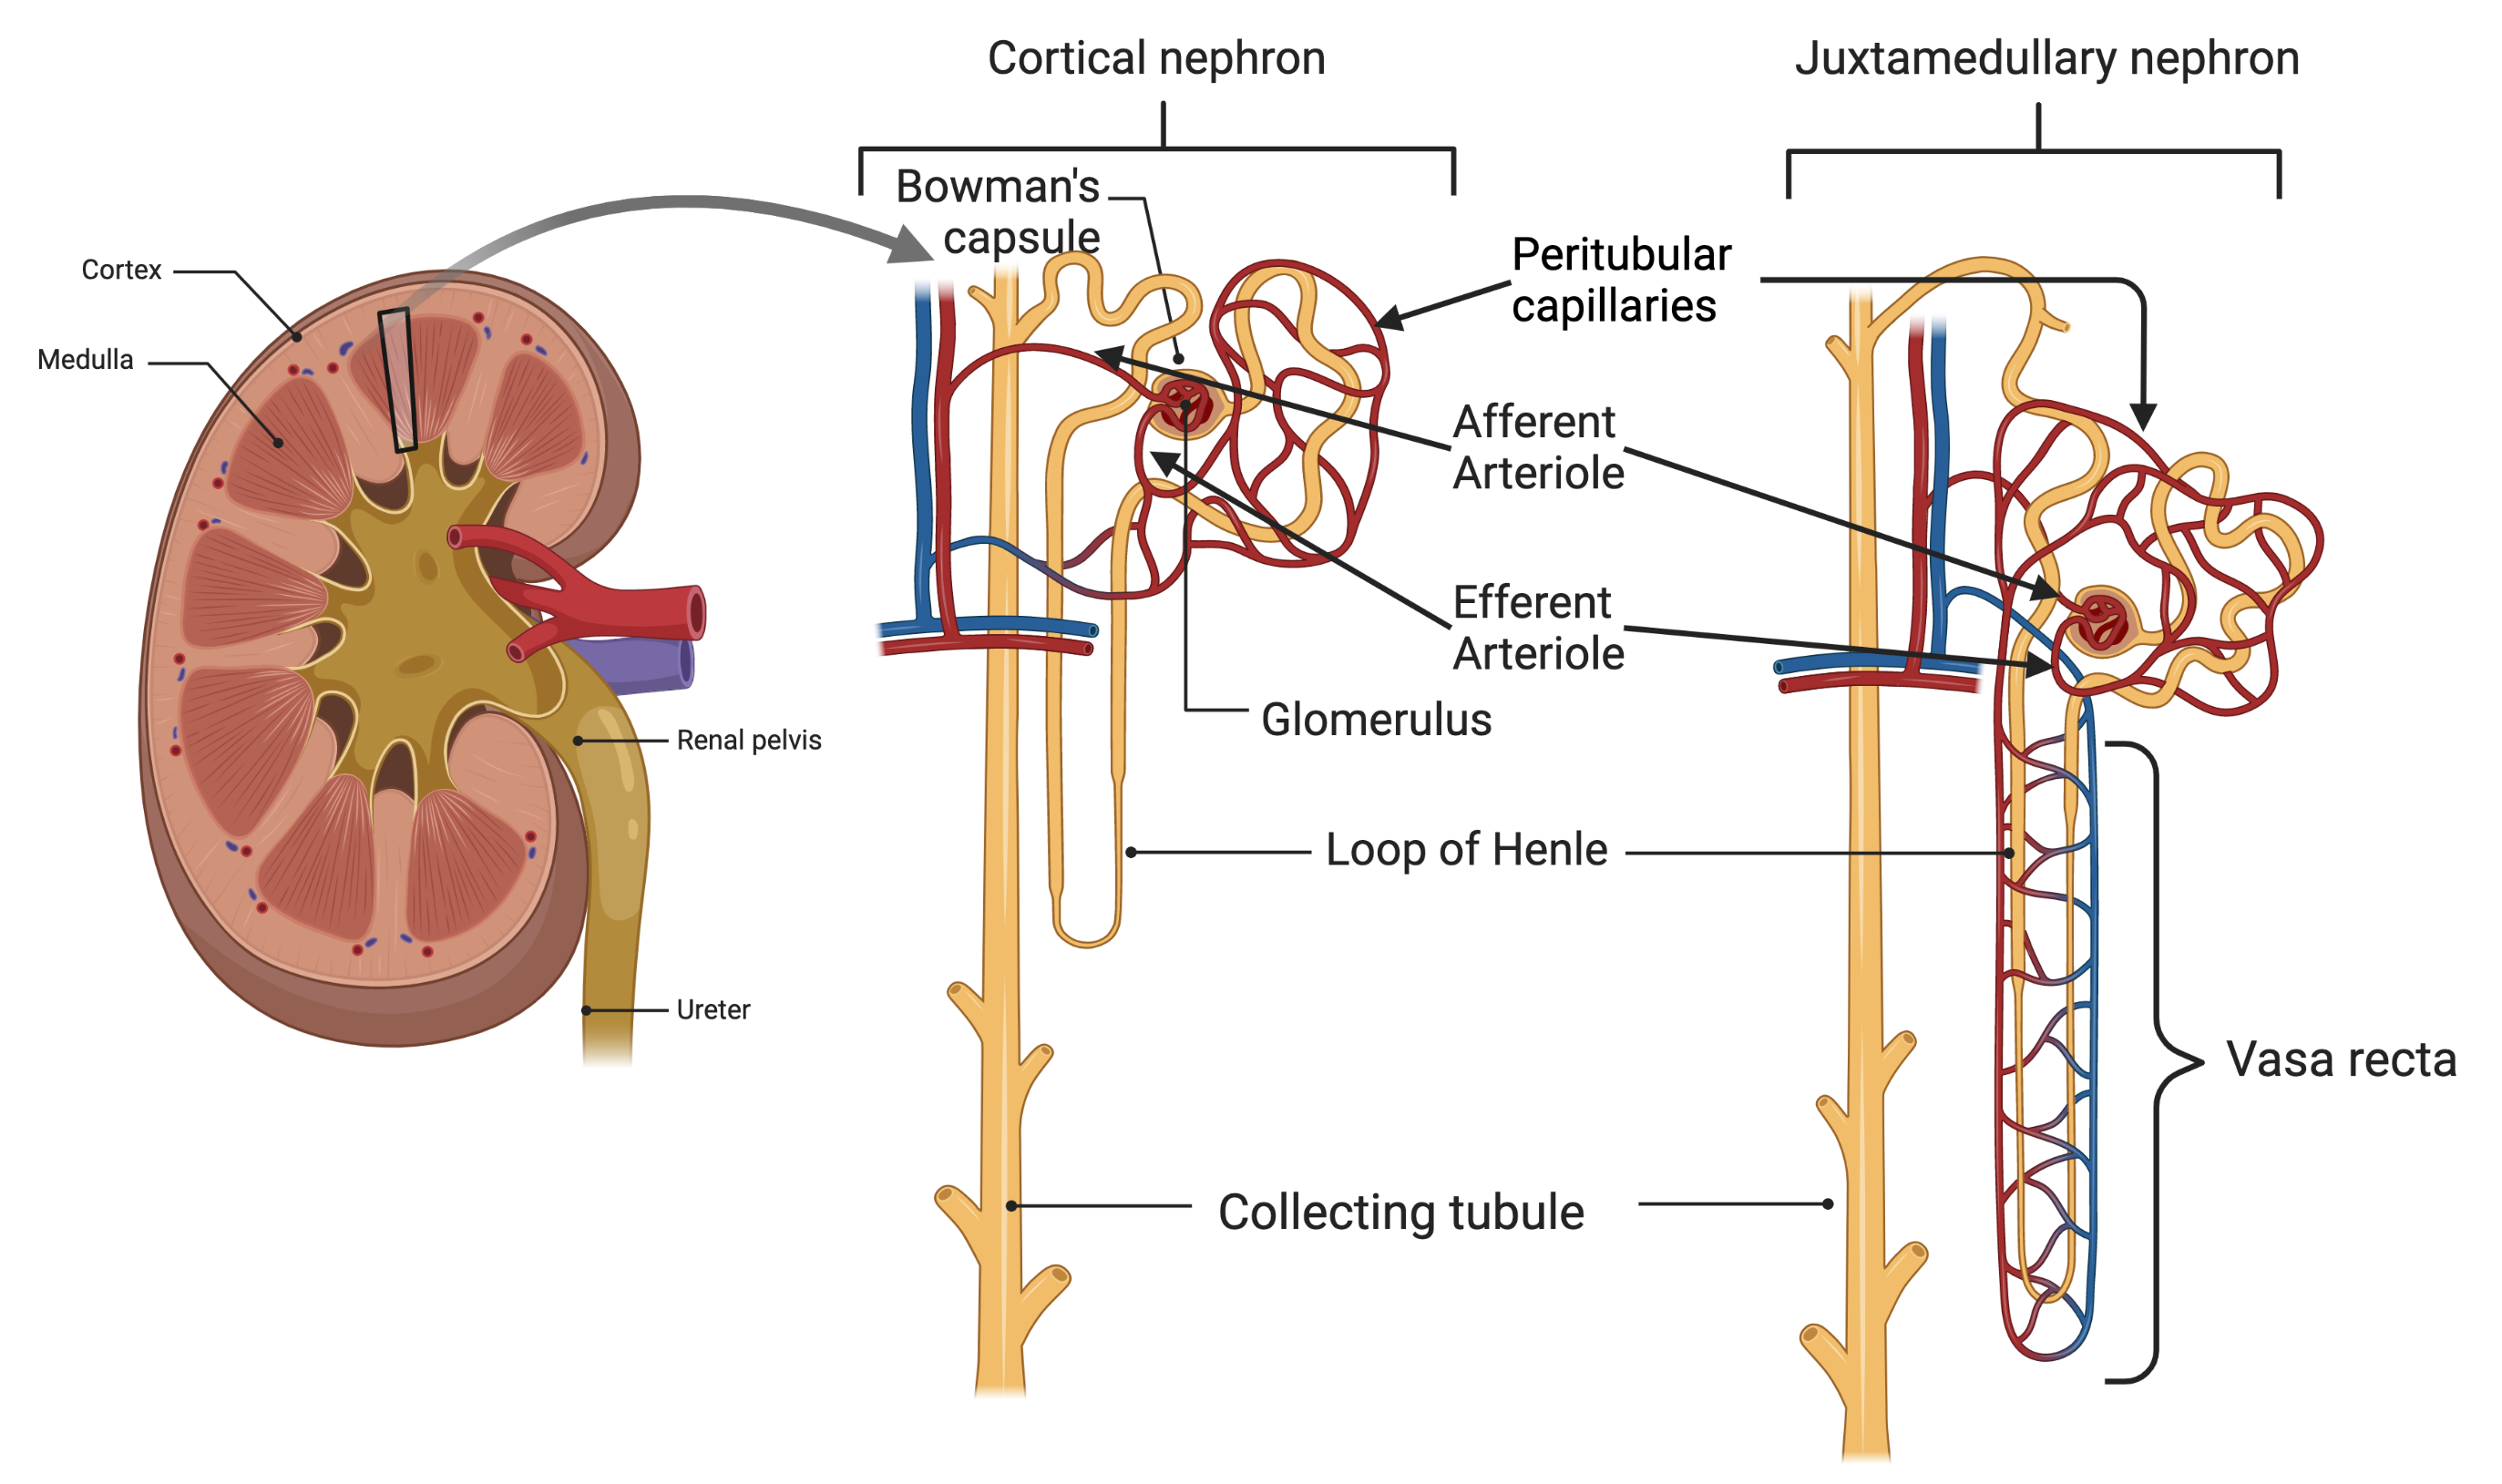
\includegraphics[width=1.0\linewidth]{./figure/Kidney_Anatomy.png}
    \caption{Overview of Kidney Anatomy \footnotesize{(Created with BioRender.com)}}
    \label{fig:Kidney_Anatomy}
\end{figure}  


From this region the ultrafiltrate (which will become urine) travels through a looping tubular structure that serve the functions of re-absorption and secretion. The segments of the nephron tubule that emerge from Bowman’s capsule includes several distinct functional units (in order): the proximal convoluted tubule, the proximal straight tubule, the loop of Henle (which contains a thin descending limb, a thin ascending limb, and a thick ascending limb), the distal convoluted tubule, and the collecting ducts. The distinct reabsorption and secretion functions across the tubule are based on a highly specialized epithelial cells lining each segment. The collecting ducts drain regionally into pouches which then drain larger pouches eventually reaching the renal pelvis which proceed into the ureter. Through this collecting duct system the urine from each kidney drains into a ureter and is transported to the bladder for storage and eventual elimination.

There are two types of nephrons, superficial cortical nephrons and juxtamedullary nephrons, which are distinguished by the location of their glomeruli and the length of their loops of Henle. The superficial cortical nephrons have their glomeruli in the outer cortex (which is more superficial) and have relatively short loops of Henle. The juxtamedullary nephrons have their glomeruli deeper in the kidney with larger glomeruli and therefore have higher glomerular filtration rates. The juxtamedullary nephrons also have long loops of Henle that go deep into the kidney that are essential for the concentration of urine. 

\paragraph{Renal Blood Vessels}
A unique aspect to renal blood vessels is that they have two sets of arterioles. Blood enters each kidney though the renal artery, which branches until the smallest arteries subdivide into the first set of arterioles, the afferent arterioles. The afferent arterioles function to deliver blood to the glomerular capillaries - a major site of filtration in the nephron. Following ultrafiltration blood travels through the second set of arterioles, the efferent arterioles, which deliver blood to the peritubular capillaries, a major site for water and solute reabsorption. Having arterioles before and after the glomerulus equips each nephron with a unique ability to regulate the hydrostatic pressure of the glomerular capillaries (PG), resulting in changes to both renal blood flow and glomerular filtration rate. For example, constriction at either the afferent or efferent end of the glomerulus will result in an increased vascular resistance and subsequently a reduced renal blood flow (explained by Poiseuille’s Law in Chapter \ref{chp:circulation}, Equation \ref{Poiseuille}). This concept will be further explored later in the chapter. 
To further assist in homeostatic regulation of water-solute balance, the juxtamedullary nephrons and more specifically, the peritubular nephrons have specialized capillary loops called Vasa Recta. These blood vessels travel in a similar form to the Loop of Henle and act as osmotic exchanges, which regulate urine concentration upon excretion. 


\subsection{Renal Clearance}

Renal clearance is the volume of plasma cleared of a substance per unit time and is determined by filtration, reabsorption and secretion. Substances with the highest clearances are both filtered and secreted and may be completely removed on a single pass of blood through the kidneys. Substances with the lowest clearances either are not filtered or are filtered and subsequently reabsorbed and may not be removed at all.  Renal clearance is based on the rate substances are removed (cleared) from plasma in the kidneys.

The higher the renal clearance, the more plasma that is cleared of the substance. The equation for renal clearance is as follows:
\vspace{4mm}
\begin{equation}
    C_x (mL/min) = \frac{U_x \times \dot{V}}{P_x}
    \label{renal_clearance}
\end{equation}

\vspace{4mm}

\begin{itemize}
    \item $C_x$ ($mL/min$) is renal clearance for any substance $x$
    \item $U_x$ ($mg/mL$) is the concentration of substance $x$ in the urine
    \item $\dot{V}$ ($mL/min$) is the flow rate (urine volume / time)
    \item $P_x$ ($mg/mL$) is the concentration of substance $x$ in the plasma
\end{itemize}

All together renal clearance is the ratio of urinary excretion to plasma concentration. For a given plasma concentration, renal clearance of a substance increases as the urinary excretion increases. The units of clearance are volume per unit time, which is the volume of plasma cleared of the substance per unit time ($mL/min$, $mL/hour$. $mL/day$, etc).

\paragraph{Renal Clearance Example}

An important point about renal clearance is that the volume of plasma cleared of substance ($x$) is mixed with the remainder of the plasma \cite{richardson_addressing_2004}. If urine was collected for an entire day and the $mmol/L$ of $Na^+$ is measured in the urine and the plasma (therefore the entire ECF) we can solve Equation \ref{renal_clearance}:

\vspace{4mm}

\begin{equation}
    C_{Na^+} (mL/day) = \frac{[Na^+]_{U} \times \dot{V}}{[Na^+]_{P}}
    \label{Na_Clearance}
\end{equation}

\vspace{4mm}

Entering measured values:

\vspace{4mm}

\begin{equation}
    C_{Na^+} (mL/day) = \frac{100 mmol/L \times 2000 mL/day}{140 mmol/L}
    \label{Na_Clearance_Example}
\end{equation}

\vspace{4mm}

In Equation \ref{Na_Clearance_Example}, $C_{Na^+} = 1428 mL/day$, which means 1428 $mL/day$ of plasma was cleared of $Na^+$ on that day. Since $Na^+$ must be balanced a nearly equal amount of $Na^+$ must have been ingested and absorbed. If plasma is 5712 $mL$ (an approximate but physiologically viable estimate for a person weighing 100 kg that makes this calculation easier), then $\frac{1}{4}$ of the plasma was cleared of $Na^+$. If $Na^+$ was not ingested and absorbed then the ECF $Na^+$ would drop to 105 $mmol/L$ (outside of the lethal limits (See Table \ref{table:ecf_value_ranges})). For $Na^+$ to stay at 140 $mmol/L$ in 5714 $mL$ of plasma would require approximately 800 $mg$ of $Na^+$ to be ingested and absorbed.\footnotemark\footnotetext{$mg$ to $mmol$ conversion completed at \url{http://www.nafwa.org/convert1.php}}
Thankfully the kidneys regulate the renal clearance of $Na^+$ to match what is actually absorbed so that people do not have to adjust what they ingest, which would require the constant measurement of $Na^+$ in the urine and the above calculations.\footnotemark\footnotetext{The reader is not expected to be able to replicate the above example, it is provided to assist understanding of renal clearance.} In situations of reduced or impaired renal function dietary modification of $Na^+$ may be necessary. The general principle here is that normal physiology affords individuals lots of freedom with its ability to make adjustments to buffer the consequences of behavior. As that physiological capacity is lost with aging and various chronic conditions, behavior must be adjusted to avoid the consequences. 

\paragraph{Renal Clearance of Substances}

The renal clearance of any substance is related to how that substance is handled by the kidneys through the processes of filtration, reabsorption and secretion. Renal clearance of albumin is approximately zero because albumin is not filtered. The renal clearance of glucose is also zero. Glucose is filtered and then completely reabsorbed. $Na^+$, urea, phosphate, and $Cl^-$ have clearances that are higher than zero because they are filtered and then partially, and selectively, reabsorbed as required. Inulin, a fructose sugar, is a special case that has made it valuable in the study of kidney function. Inulin is freely and completely filtered across the glomerular capillaries and it is neither reabsorbed nor secreted. Therefore the amount of inulin in the urine is the amount that was filtered. Its clearance measures the glomerular filtration rate (GFR) and has been utilized as the gold standard for identifying other useful measures of the GFR.

\subsubsection{Urine Formation \& Excretion by Micturition}

Urine is formed by anything (including water) that is filtered and not reabsorbed, or not filtered and then secreted. Urine leaves the kidneys and flows through the ureters into the bladder. Peristaltic contractions of smooth muscles in the ureter, enhanced by parasympathetic activation, force urine from the kidneys toward the bladder which help maintain the flow of urine from the kidneys even as pressure rises in the bladder. 

The bladder is a smooth muscle chamber with two parts. The bladder body collects urine and the neck is a funnel-shaped extension that connects with the urethra. The smooth muscle of the bladder can increase bladder pressure to 40-60 $mm Hg$ and play a major role in emptying the bladder during micturition.

The smooth muscle of the bladder wall is influenced by the autonomic nervous system and a spinal cord stretch reflex. Micturition is the process of emptying the bladder when it is filled. Filling of the bladder increases its pressure and therefore wall tension rises. Pelvic nerves connect with the spinal cord through the sacral plexus include sensory and motor nerve fibers. The sensory nerve fibers detect when the bladder wall tension rises above a threshold level that activates the micturition reflex to empty the bladder or, if this fails, creates a conscious desire to urinate. The motor nerves transmitted to the pelvic nerves are parasympathetic fibers.

The bladder neck includes the internal sphincter muscle interlaced with a large amount of elastic tissue. The natural tone of the internal sphincter muscle keeps the bladder from emptying until the pressure in the main part of the bladder rises above a critical threshold. Beyond the neck of the bladder the urethra passes through the urogenital diaphragm, which includes a layer of muscle called the external sphincter. This muscle is a voluntary skeletal muscle and is used to prevent urination even when the micturition reflex is attempting to empty the bladder.

\paragraph{Urinary Incontinence}

There are numerous potential causes of urinary incontinence. A common cause of all forms includes the inability to prevent bladder pressure, either through the micturition reflex or external provocations such as abdominal pressure creating bladder pressure (for example during coughing, laughing, valsalva, etc), from resulting in urination. Of course that statement is as useful to treatment of incontinence as saying the common cause of all falls is gravity. The micturition reflex includes a complete cycle of (1) progressive and rapid increase in bladder pressure, (2) sustained increase in bladder pressure, and (3) return of the pressure to the basal tone of the bladder. 
\vspace{4mm}
The steps include \cite{hall_guyton_2020}:

\begin{enumerate}
    \item Sensory signals from the bladder wall stretch receptors are conducted to sacral segments of the spinal cord through the pelvic nerves and then reflexively back to the bladder through the parasympathetic nerves by way of the pelvic nerves.
    \item  Once the micturition reflex is sufficiently powerful, it causes another reflex that passes through the pudendal nerves to the external sphincter to inhibit it. If this inhibition is more potent than the voluntary constrictor signals to the external sphincter, urination occurs.
    \item  The micturition reflex is an autonomic spinal cord reflex, but it can be inhibited or facilitated by centers in the brain stem, mainly the pons, and several centers in the cerebral cortex that are mainly excitatory but can become inhibitory.
\end{enumerate}

Not urinating includes the collaborative function of the internal and external sphincter. Both are involved in the micturition reflex above. When the micturition reflex is sufficiently powerful, either due to increased urine volume increasing wall tension, or increased abdominal pressure including bladder pressure and increasing wall tension, voluntary tone of the external sphincter must be properly timed and sufficient to prevent urination. Much of Women's Health Physical Therapy is centered on helping post-partum women regain voluntary control over the micturition reflex. It is important to point out that the terminology "voluntary" simply means a voluntary skeletal muscle. It does not necessarily mean conscious control. For example, several voluntary skeletal muscles are involved when you breath, maintain a particular posture or walk that while being voluntary are not conscious (you can think about your breathing, posture and walking muscle activation, but you typically do not).


\subsection{Glomerular Filtration}

Glomerular filtration is the first step in the formation of urine. The rate of glomerular filtration is appropriately called the glomerular filtration rate (GFR). As blood enters the glomerular capillaries, a portion of that blood is filtered into Bowman’s capsule. The fluid that is filtered is similar to interstitial fluid and at this point is called an ultrafiltrate. Ultrafiltrate contains water and all of the small solutes of blood, but not proteins and blood cells. The pressures responsible for glomerular filtration are similar to the pressures operating for micro-circulation filtration in systemic capillaries (Chapter \ref{chp:ecf_microcirculation}). However, the characteristics and surface area of glomerular capillaries result in a much higher GFR than filtration in systemic capillaries (glomerular capillaries have a higher $K_f$ than systemic circulation capillaries). Also, unlike filtration in systemic circulation which renters the same capillary that it had been filtered out of, the ultrafiltrate of glomerular filtration renters the peritubular capillaries through reabsorption and can be more selective. The ultrafiltrate that does not re-enter the vascular fluid does not enter lymph vessels, but rather proceeds through the renal tubules for urine formation and excretion.

Recall that there are four pressures for filtration, two hydrostatic pressures (one in capillary blood and one in interstitial fluid) and two osmotic pressures (one in capillary blood and one in interstitial fluid). Applying these pressures to glomerular capillaries, there is one small modification because the osmotic pressure of Bowman’s capsule is considered to be zero and therefore is not included in the equation for GFR \cite{costanzo_physiology_2013}:

\begin{equation}
GFR = K_f \times (P_{G} - P_{B} - \pi_{G})
\label{GFR}
\end{equation}

\begin{itemize}
\item $GFR$ = Glomerular filtration rate ($mL/min$) 
\item $K_f$ = Filtration coefficient ($mL/min \cdot mm Hg$) 
\item $P_{G}$ = Hydrostatic pressure in glomerular capillary ($mm Hg$) 
\item $P_{B} $= Hydrostatic pressure in Bowman’s capsule ($mm Hg$) 
\item $\pi_{G}$ = Osmotic pressure in glomerular capillary ($mm Hg$) 
\end{itemize} 

The glomerular $K_f$  is the water permeability of the glomerular capillary wall. Two factors that contribute to $K_f$ are the water permeability per unit of surface area and the total surface area. $K_f$ for glomerular capillaries is approximately 100-fold greater than systemic capillaries (such as skeletal muscle capillaries) because of the combination of a higher total surface area and a higher intrinsic water permeability. The consequence of this extremely high $K_f$ is that much more fluid is filtered from glomerular capillaries than from other capillaries. $K_f$ is decreased with damage to the glomerular capillaries brought on by chronic conditions such as diabetes and high blood pressure (hypertension (HTN)).

The $P_{G}$ is a pressure favoring filtration.  Compared with systemic capillaries, $P_{G}$ is relatively high (60 $mm Hg$). In systemic capillaries, hydrostatic pressure falls along the length of the capillary; in glomerular capillaries, it remains constant along the entire length. This is possible because $P_{G}$ is regulated with two sets of arterioles, those entering the glomerular capillaries (afferent arterioles) and those exiting the glomerular capillaries (the efferent arterioles). This regulatory system also allows for $P_{G}$  to remain relatively constant across a wide range of blood pressures (80-200 $mm Hg$).

The $P_{B}$ is a pressure opposing filtration. The origin of this pressure (18 $mm Hg$) is the fluid present in Bowman’s capsule and the tubule of the nephron.

The $\pi_{G}$ is a pressure opposing filtration. $\pi_{G}$ is determined primarily by the protein concentration of glomerular capillary blood. $\pi_{G}$ progressively increases along the capillary length as fluid (but not protein) is filtered out of the capillary. $\pi_{G}$ eventually increases to the point where net filtration pressure becomes zero and glomerular filtration stops (filtration equilibrium). 

The net filtration pressure (nfp) in glomerular capillaries always favors filtration so the direction of fluid movement is always out of the capillaries. The greater the net pressure, the higher the GFR.


\begin{figure}[!h]
    \centering
    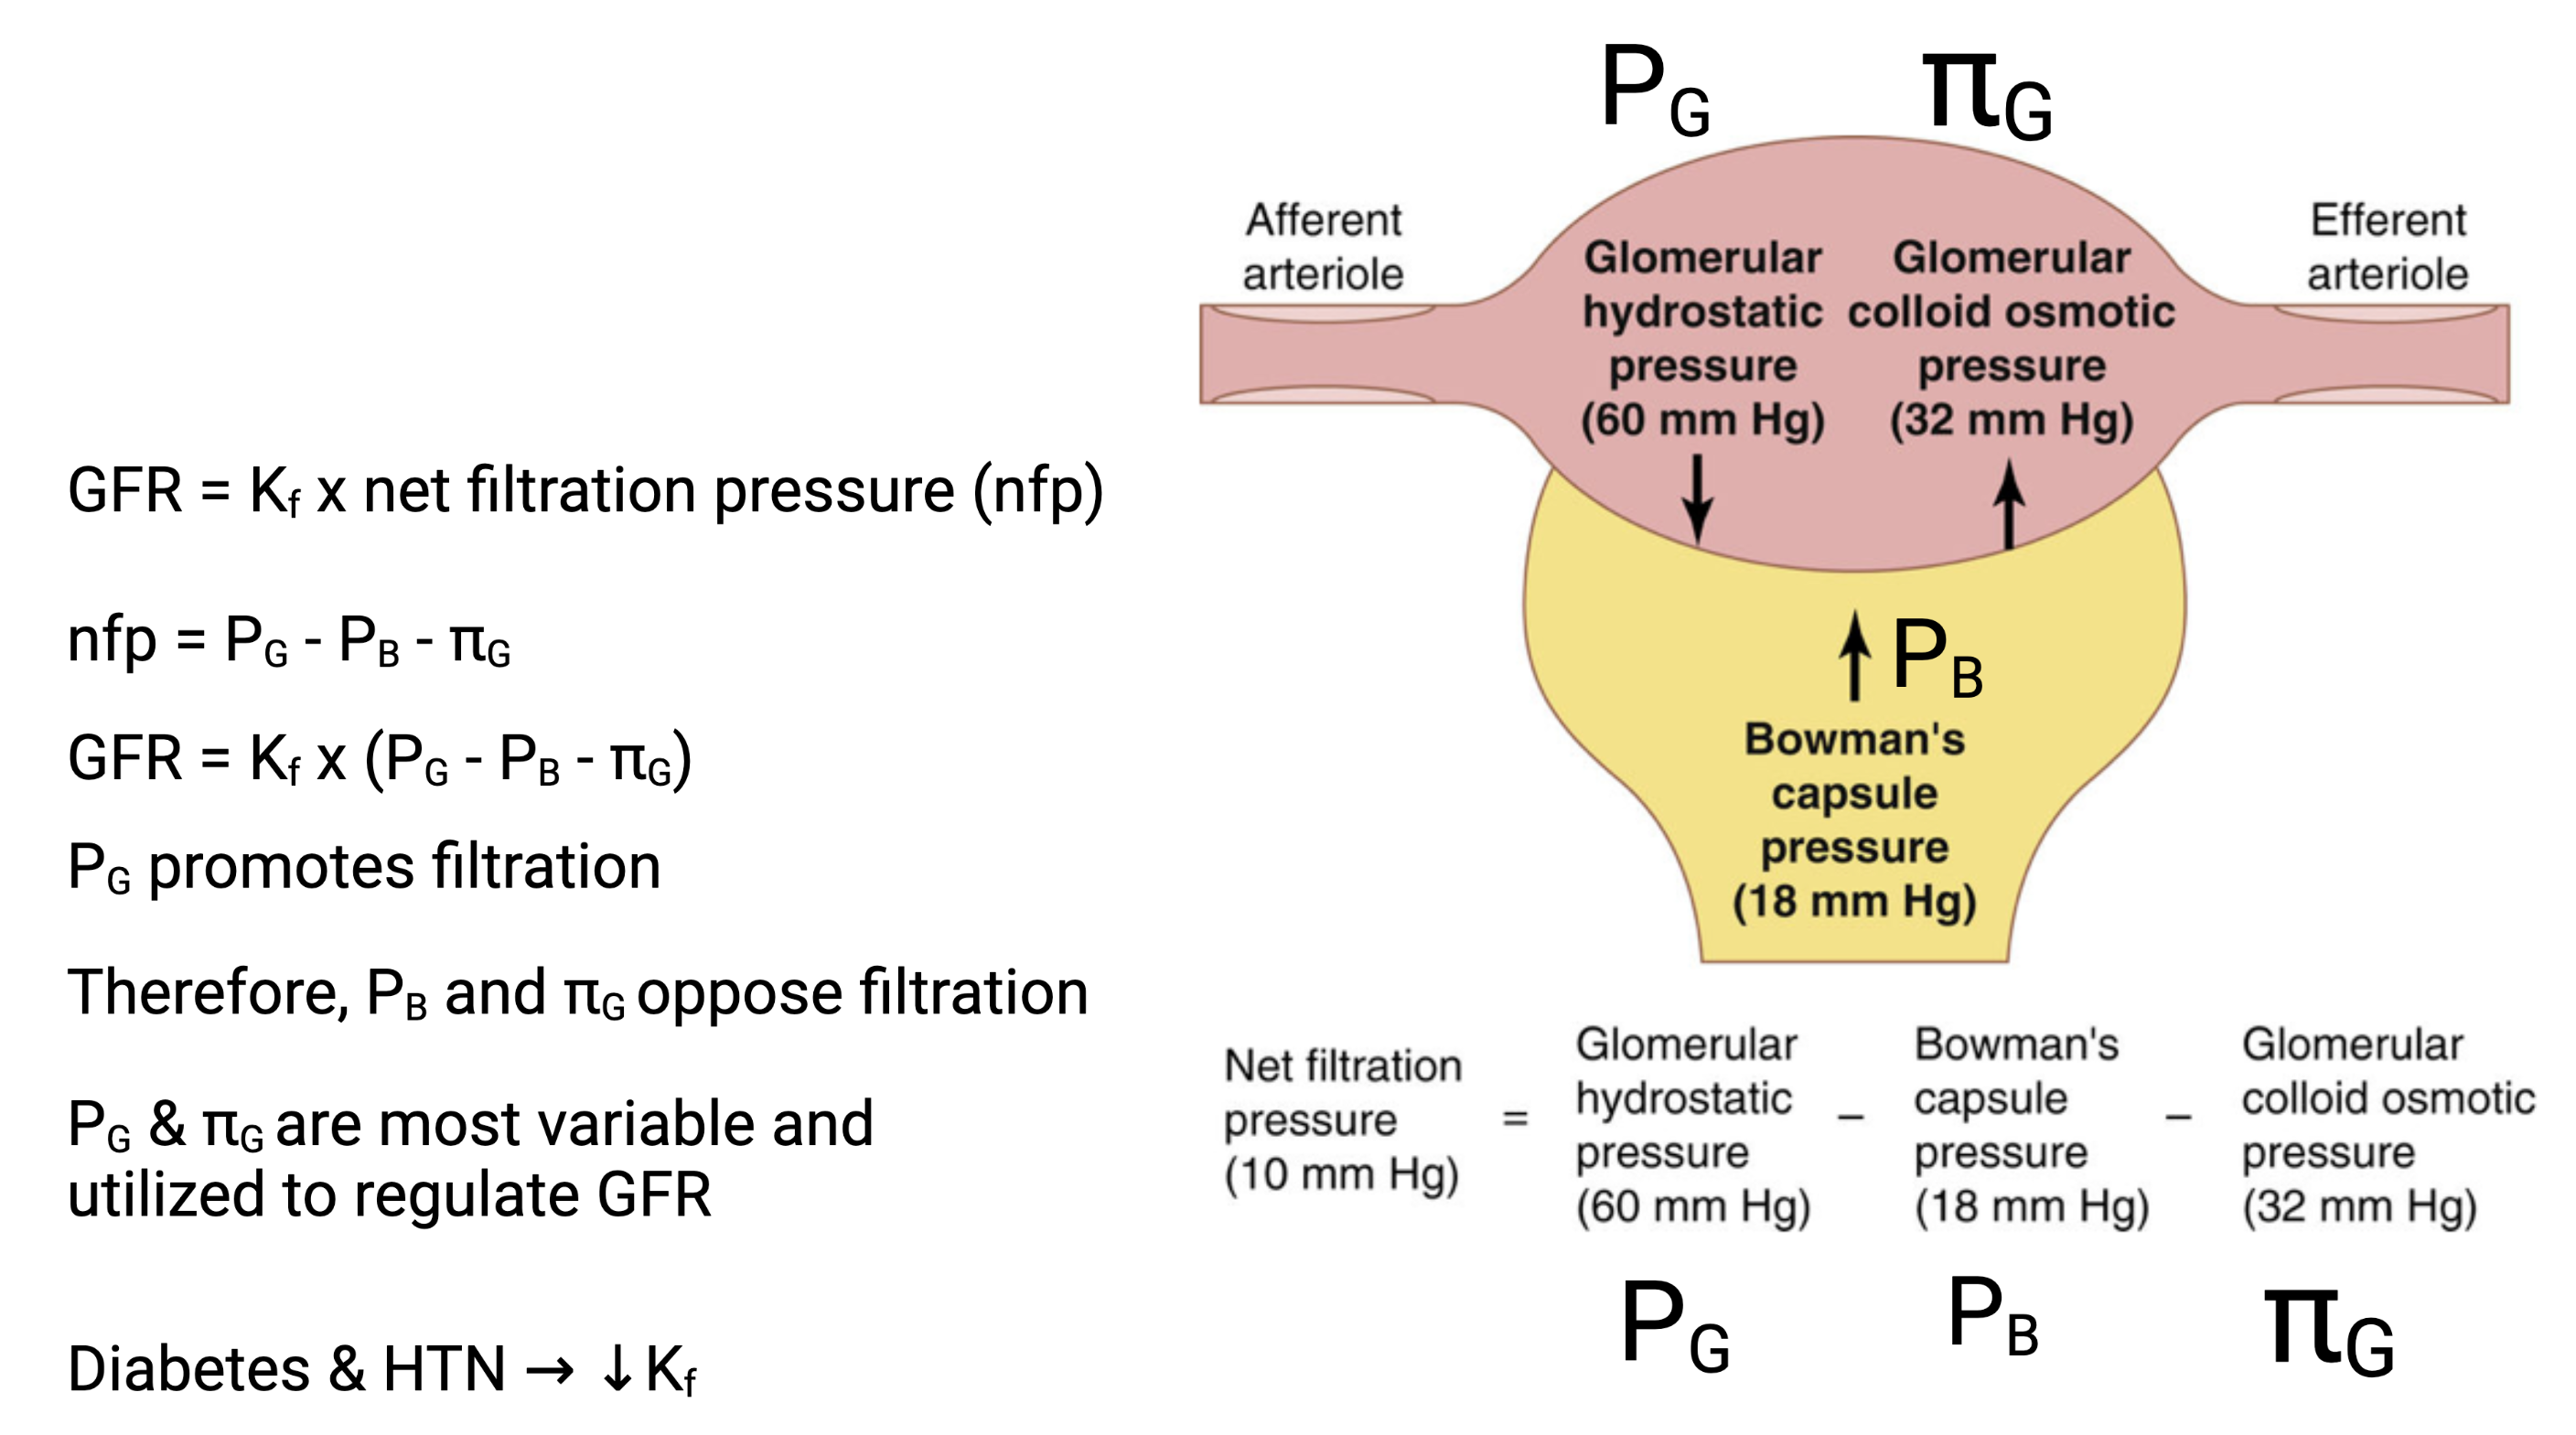
\includegraphics[width=1\linewidth]{./figure/RBF_GFR.png}
    \caption{Filtration Pressures of the Glomerular Filtration Rate \footnotesize{(Created with BioRender.com)}}
    \label{fig:RBF_GFR}
\end{figure}

Figure \ref{fig:RBF_GFR} presents of the three pressures represented by arrows and summarizes the equations. The direction of the arrow indicates whether the pressure favors filtration out of the capillary or absorption into the capillary. The size of the arrow indicates the relative magnitude of the pressure. The numerical value of the pressure ($mm Hg$) has a plus sign if the pressure favors filtration and a minus sign if the pressure favors absorption. The net filtration pressure (nfp) is the sum of the three pressures.

\paragraph{Changes in $P_{G}$}

Changes in $P_{G}$ are produced by changes in the resistance of the afferent and efferent arterioles which subsequently change renal blood flow (RBF). Changes in GFR depend on changes to $P_{G}$ which depend on how both the afferent and efferent arterioles are affected.

Constriction of the afferent arteriole increases afferent arteriole resistance and decreases renal blood flow (RBF). GFR also decreases because, as less blood flows into the glomerular capillary $P_{G}$ decreases, reducing net ultrafiltration pressure.

Constriction of the efferent arteriole increases efferent arteriole resistance. The effect of efferent arteriole constriction on RBF is the same as with constriction of the afferent arteriole (decreases), yet the effect on GFR is opposite (increases). GFR increases because blood is restricted from leaving the glomerular capillary, causing $P_{G}$ and nfp to increase.

\paragraph{Effects of Angiotensin II}

Levels of angiotensin II constricts both afferent and efferent arterioles with an inverse but preferential effect on efferent arterioles. Efferent arterioles constrict inversely proportional to angiotensin II, and afferent arterioles constrict proportional to angiotensin II. Therefore, a low level of angiotensin II has a large constrictor effect on efferent arterioles and a small constrictor effect on afferent arterioles. This decreases RBF but increases GFR due to an elevated $P_G$ despite the decreased RBF. A higher level of angiotensin II has a medium constrictor effect on efferent arterioles and a medium constrictor effect on afferent arterioles, leading to a decrease in RBF with a smaller (than expected by the reduction in RBF) decrease in GFR. Thus, with both low and high, but normal range, levels of angiotensin II, because of its preferential effect on efferent arterioles, the GFR is preserved in the setting of vasoconstriction. In the setting of higher than normal range angiotensin II there is less constriction of efferent arterioles with moderate to high constriction of afferent arterioles. This situation results in reduced RBF and reduced GFR due to reduced  $P_{G}$.

\paragraph{Changes in $\pi_{G}$}
Changes in $\pi_{G}$ are produced by changes in plasma protein concentration. Increases in plasma protein concentration produce increases in $\pi_{G}$, which decrease the nfp and GFR. Decreases in plasma protein concentration produce decreases in $\pi_{G}$ which increase both net filtration pressure and GFR.

\paragraph{Changes in $P_{B}$}
Changes in $P_{B}$ can be produced by obstructing urine flow (e.g., ureter stone or constriction). If the ureter is constricted, urine cannot flow through that ureter to the bladder, causing urine to back up in the kidney. Consequently, hydrostatic pressure in the nephrons will increase as far back as Bowman’s capsule, producing an increase in $P_{B}$. An increase in $P_{B}$ decreases the nfp, thereby decreasing GFR. 


\subsubsection{Clinical Estimation of GFR}

The clinical estimation of GFR provides an overall assessment of renal function. As previously mentioned, inulin is freely and completely filtered across the glomerular capillaries and it is neither reabsorbed nor secreted. Therefore the amount of inulin in the urine is the amount that was filtered. Its clearance measures the GFR. Inulin has been utilized as the gold standard for identifying other useful measures of the GFR. The use of inulin to measure GFR requires a prolonged highly controlled situation that includes set infusion of inulin and collection of urine for hours to record its clearance. Therefore, inulin is rarely utilized clinically to measure GFR.

\paragraph{BUN and creatinine}

The closest substance to inulin for estimation of GFR is is creatinine. It is freely filtered across the glomerular capillaries but is also secreted to a small extent. Therefore, clearance of creatinine slightly overestimates the GFR. However, since creatinine is an endogenous substance it does not need to be infused in order to estimate GFR. Urea is another endogenous substance that does not need to be infused that is filtered across the glomerular capillaries. Together, blood urea nitrogen (BUN) and serum creatinine concentration are used to estimate GFR because each substance depends on the filtration step in order to be excreted in urine and they are reabsorbed (urea) in small quantities, or secreted in small quantities. 

With a decrease in GFR due to renal conditions (such as renal failure), BUN and serum creatinine both increase because they are not adequately filtered. But with lower blood volume (hypovolemia, due to dehydration) or reduced RBF (perfusion, due to heart failure) there is also decreased GFR and both BUN and serum creatinine are increased. However, because urea is reabsorbed and creatinine is not, BUN increases more than serum creatinine. Therefore an indicator of hypovolemia or heart failure caused renal insufficiency is an increased ratio of BUN/creatinine to more than 20. While renal failure due to renal causes produces an increase in both BUN and serum creatinine, it does not produce an increase in the BUN/creatinine ratio \cite{hall_guyton_2020}.



\subsection{Tubular Reabsorption}

Glomerular filtration results in the production of large quantities of ultrafiltrate each day (approximately  180 L/day). If all of this ultrafiltrate were excreted as urine the following quantities would be lost each day: 180 $L$ of water; 25,200 $mmol$ of $Na^+$; 19,800 $mmol$ of $Cl^-$; 4320 $mmol$ of $HCO_{3}^{-}$; and 14,400 $mg$ of glucose. Each of these losses is 10 times more than the amount present in the entire ECF. This is clearly not a sustainable approach to mass balance. 

There are a set of reabsorption mechanisms in the epithelial cells lining the renal tubule that return these (and other) substances to the peritubular capillaries, the circulation and thus to the ECF. The details of these mechanisms are beyond the scope of this text. Overall, reabsorption includes the return to capillaries through several different transport proteins that either selectively and directly transport substances, or through the transport of substances which then manipulate the osmolarity between the renal tubule and the peritubular capillaries.  Water and many solutes ($Na^+$, $Cl^-$, $HCO_3^-$, glucose, amino acids, urea, $Ca^{2+}$, $Mg^{2+}$, phosphate, lactate, and citrate) are reabsorbed from ultrafiltrate back into the peritubular capillaries. If reabsorption did not occur, most of these constituents of ECF would be rapidly lost in the urine.

This approach, the generation of a large quantity of ultrafiltrate and the selective reabsorption back into the capillaries, is a highly efficient way to filter and clear waste products (urea, creatinine that have limited reabsorption), and regulate the blood and ECF content of other substances. For example, even though glucose is filtered and then reabsorbed, in certain hyperglycemic situations with diabetes, glucose cannot be fully reabsorbed which results in glucose in the urine (glycosuria).  Glycosuria contributes to an upper limit of blood glucose and its acutely deleterious effects, but it is not a healthy long term homeostatic mechanism for glucose control. 

Reabsorption, very generally, is adjusted based on ECF fluid volume. Increased ECF volume inhibits tubule reabsorption which results in loss of ECF fluid volume, and decreased ECF volume stimulates tubule reabsorption which results in an increase in ECF. Different diuretics (drugs that promote water removal in urine) work at different points along the renal tubule to reduce reabsorption of water.


\subsection{Tubular Secretion}

Secretion mechanisms in the epithelial cells can remove selected and specific substances from the peritubular capillary blood and add them to urine. Organic acids, organic bases, and $K^+$ are secreted from peritubular capillary blood into tubular fluid as needed. In addition to filtration, secretion provides a mechanism for excreting substances in the urine. Compared to filtration secretion is selective like reabsorption. The secretion mechanisms involve transporters in the membranes of the epithelial cells lining the renal tubule.

\subsection{Excretion Rate}

The net reabsorption or secretion rate of a substance is the difference between its filtered load (the amount filtered) and its excretion rate. Excretion rate refers to the amount of a substance excreted per unit time. Referring back to Equation \ref{renal_clearance}, the excretion rate is related to the clearance rate. However the excretion rate is in terms of the amount of a substance excreted per time frame ($mmol/day$) whereas the clearance rate is in terms of the volume of plasma cleared of the substances ($mmol/L$). 

The filtered load of substance $x$ is equal to $GFR \times [x]_P$ (where $[x]_P$ is the plasma concentration of substance $x$). The excretion rate of a substance $x$ is equal to $\dot{V} \times [x]_U$ (where $\dot{V}$ is the rate of urine flow ($mL/day$), and $[x]_U$ is the concentration of substance $x$ in the urine). 

The excretion rate is the net result of glomerular filtration, tubular reabsorption, and tubular secretion. The excretion rate can be compared with the filtered load to determine whether a substance has been reabsorbed or secreted. The difference between the filtered load and the excretion rate is the rate of net reabsorption or net secretion. When the filtered load is greater than the excretion rate, there has been net reabsorption of the substance. If the filtered load is less than the excretion rate, there has been net secretion of the substance.
% consider adding equations and examples

\section{Renal Regulation}

Renal regulation includes both the regulation of renal function, and the renal regulation of several critical characteristics of ECF. These two aspects of regulation are highly integrated and coordinated. Renal function regulates blood volume and osmolarity by adjusting both water content and electrolytes (primarily $Na^+$). Regulation of $Na^+$ content is balanced with regulation of $Na^+$ concentration. In other words, there are limits to what the kidneys do to adjust water volume and osmolarity because they are also making sure the $Na^+$ concentration stays within fairly tight limits. The regulation of renal function is similarly based on alterations in blood volume that influence glomerular filtration, tubular reabsorption and tubular secretion. Figure \ref{fig:renal_regulation_intro} depicts the bidirectional relationship between renal blood flow (RBF), GFR and renal function (excretion rates and other functions). Renal function influences circulation and arterial pressure which then influences RBF. Arterial pressure is also regulated and is integrated with renal regulation via the hormones angiotensin II, aldosterone and anti-diuretic hormone (ADH). 

\begin{figure}[!h]
    \centering
    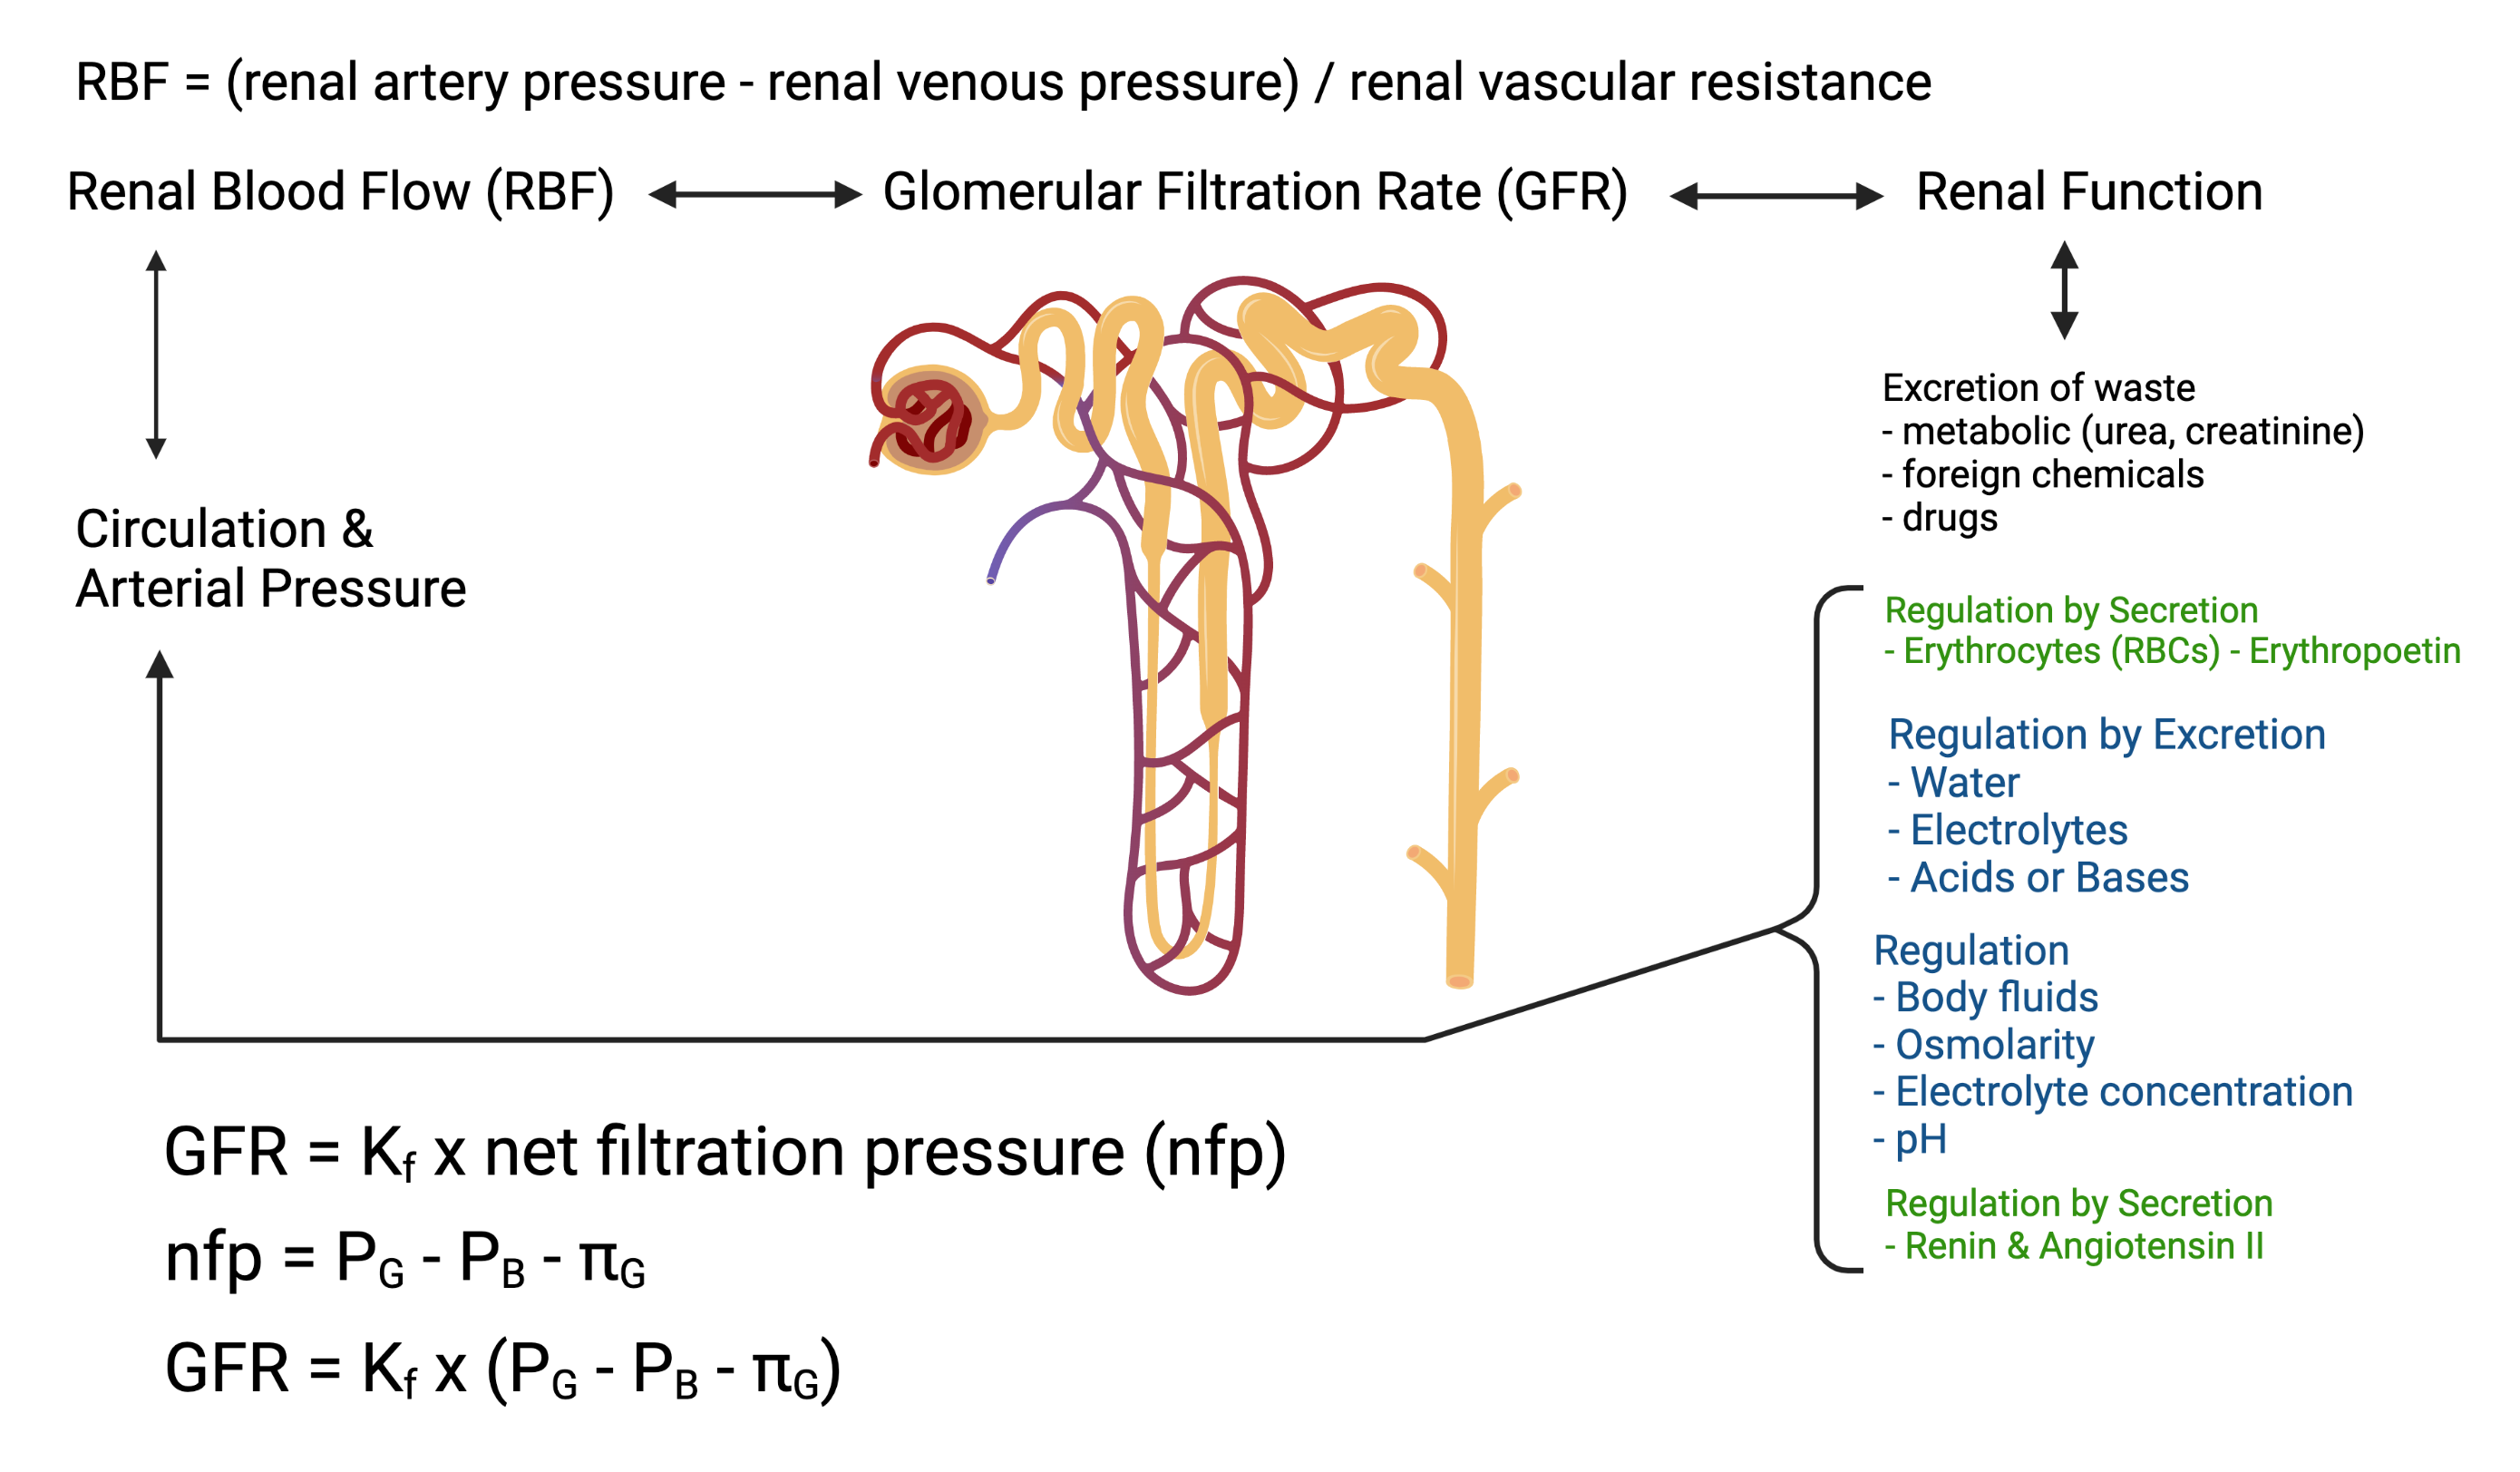
\includegraphics[width=1\linewidth]{./figure/renal_regulation_intro.png}
    \caption{Overview of Renal Regulation \footnotesize{(Created with BioRender.com)}}
    \label{fig:renal_regulation_intro}
\end{figure}


\subsection{Sodium}

The kidneys maintain a normal body $Na^+$ content by ensuring that $Na^+$ excretion equals $Na^+$ intake, a matching process called $Na^+$ balance. $Na^+$ balance is achieved by variations in the reabsorption of $Na^+$.  If $Na^+$ excretion is less than $Na^+$ intake, then there is positive $Na^+$ balance. Extra $Na^+$ is retained, primarily in the ECF. When the $Na^+$ content of ECF is increased, there is increased ECF osmolarity and thus volume; blood volume and arterial pressure also increase, and there may be edema. If $Na^+$ excretion is greater than $Na^+$ intake, then a person is in negative $Na^+$ balance. When excess $Na^+$ is lost from the body, there is a decreased $Na^+$ content of ECF, decreased ECF osmolarity and thus volume (increased ICF volume), and decreased blood volume and arterial pressure. 


\subsection{Potassium}
$K^+$ balance is maintained by shifts of $K^+$ across cell membranes and by renal regulation. The renal mechanisms for $K^+$ balance include filtration, reabsorption, and secretion. Secretion is influenced by dietary $K^+$, aldosterone, acid-base balance, and flow rate. With low $K^+$ intake, more $K^+$ is reabsorbed and less is secreted; with high $K^+$ intake less is reabsorbed and more is secreted. The secretion of  $K^+$ in the distal tubule and collecting ducts allows the fine-tuning of $K^+$ excretion to maintain $K^+$ balance.

Acid-base disturbances can effect blood $K^+$ concentration due to alterations in $K^+$ secretion. Alkalosis increases $K^+$ secretion, and acidosis decreases $K^+$ secretion. Therefore, conditions such as chronic pulmonary disease that increase blood carbon dioxide and decrease blood pH (respiratory acidosis) can be accompanied by hyperkalemia. 

Commonly used diuretics, the loop diuretics and the thiazide diuretics, cause increased $K^+$ excretion. Therefore, an important side effect of diuretic therapy is hypokalemia. The $K^+$-sparing diuretics (e.g., spironolactone, amiloride, triamterene) do not cause increased $K^+$ excretion because they inhibit all of the actions of aldosterone and inhibit $K^+$ secretion. The most common use of $K^+$-sparing diuretics is in combination with the loop or thiazide diuretics to offset hypokalemia produced by those drugs. 

\subsection{Calcium}
Calcium regulation involves kidney reabsorption in response to parathyroid hormone. However, the overall coordinated process of calcium regulation involves variations in intestinal absorption and release from bones. Therefore, it is best considered with an understanding of intestinal absorption and covered in Chapter \ref{chp:blood_nutrients} on Digestion, Absorption \& Metabolism.

\subsection{Acid Base Balance}
There are three ways the kidneys influence acid base balance. First, the secretion of $H^+$; second the reabsorption of $HCO_3^-$; and third, the production of new $HCO_3^-$. It is best to consider kidney (metabolic) causes and compensations of acid-base balance along with respiratory causes and compensations of acid-base balance. Therefore, clinical interpretation of acid-base imbalance is in Chapter \ref{chp:alveolar_oxygen} on Ventilation.


\subsection{Blood Volume \& Osmolarity}

Blood volume is regulated based on two primary factors. Its impact on BP (and through BP, RBF and subsequently GFR), and the impact of water in plasma on ECF osmolarity. These are not completely separate regulatory pathways (there is overlap). The overlap is clear when considering the integration of the hormonal mechanisms underlying the regulation of blood pressure and osmolarity. As mentioned above there are three primary hormones to be considered: angiotensin II, anti-diuretic hormone (ADH) and aldosterone. The influence of these three hormones on renal function is summarized in Figure \ref{fig:Endocrine_Regulation}.

\begin{figure}[!h]
    \centering
    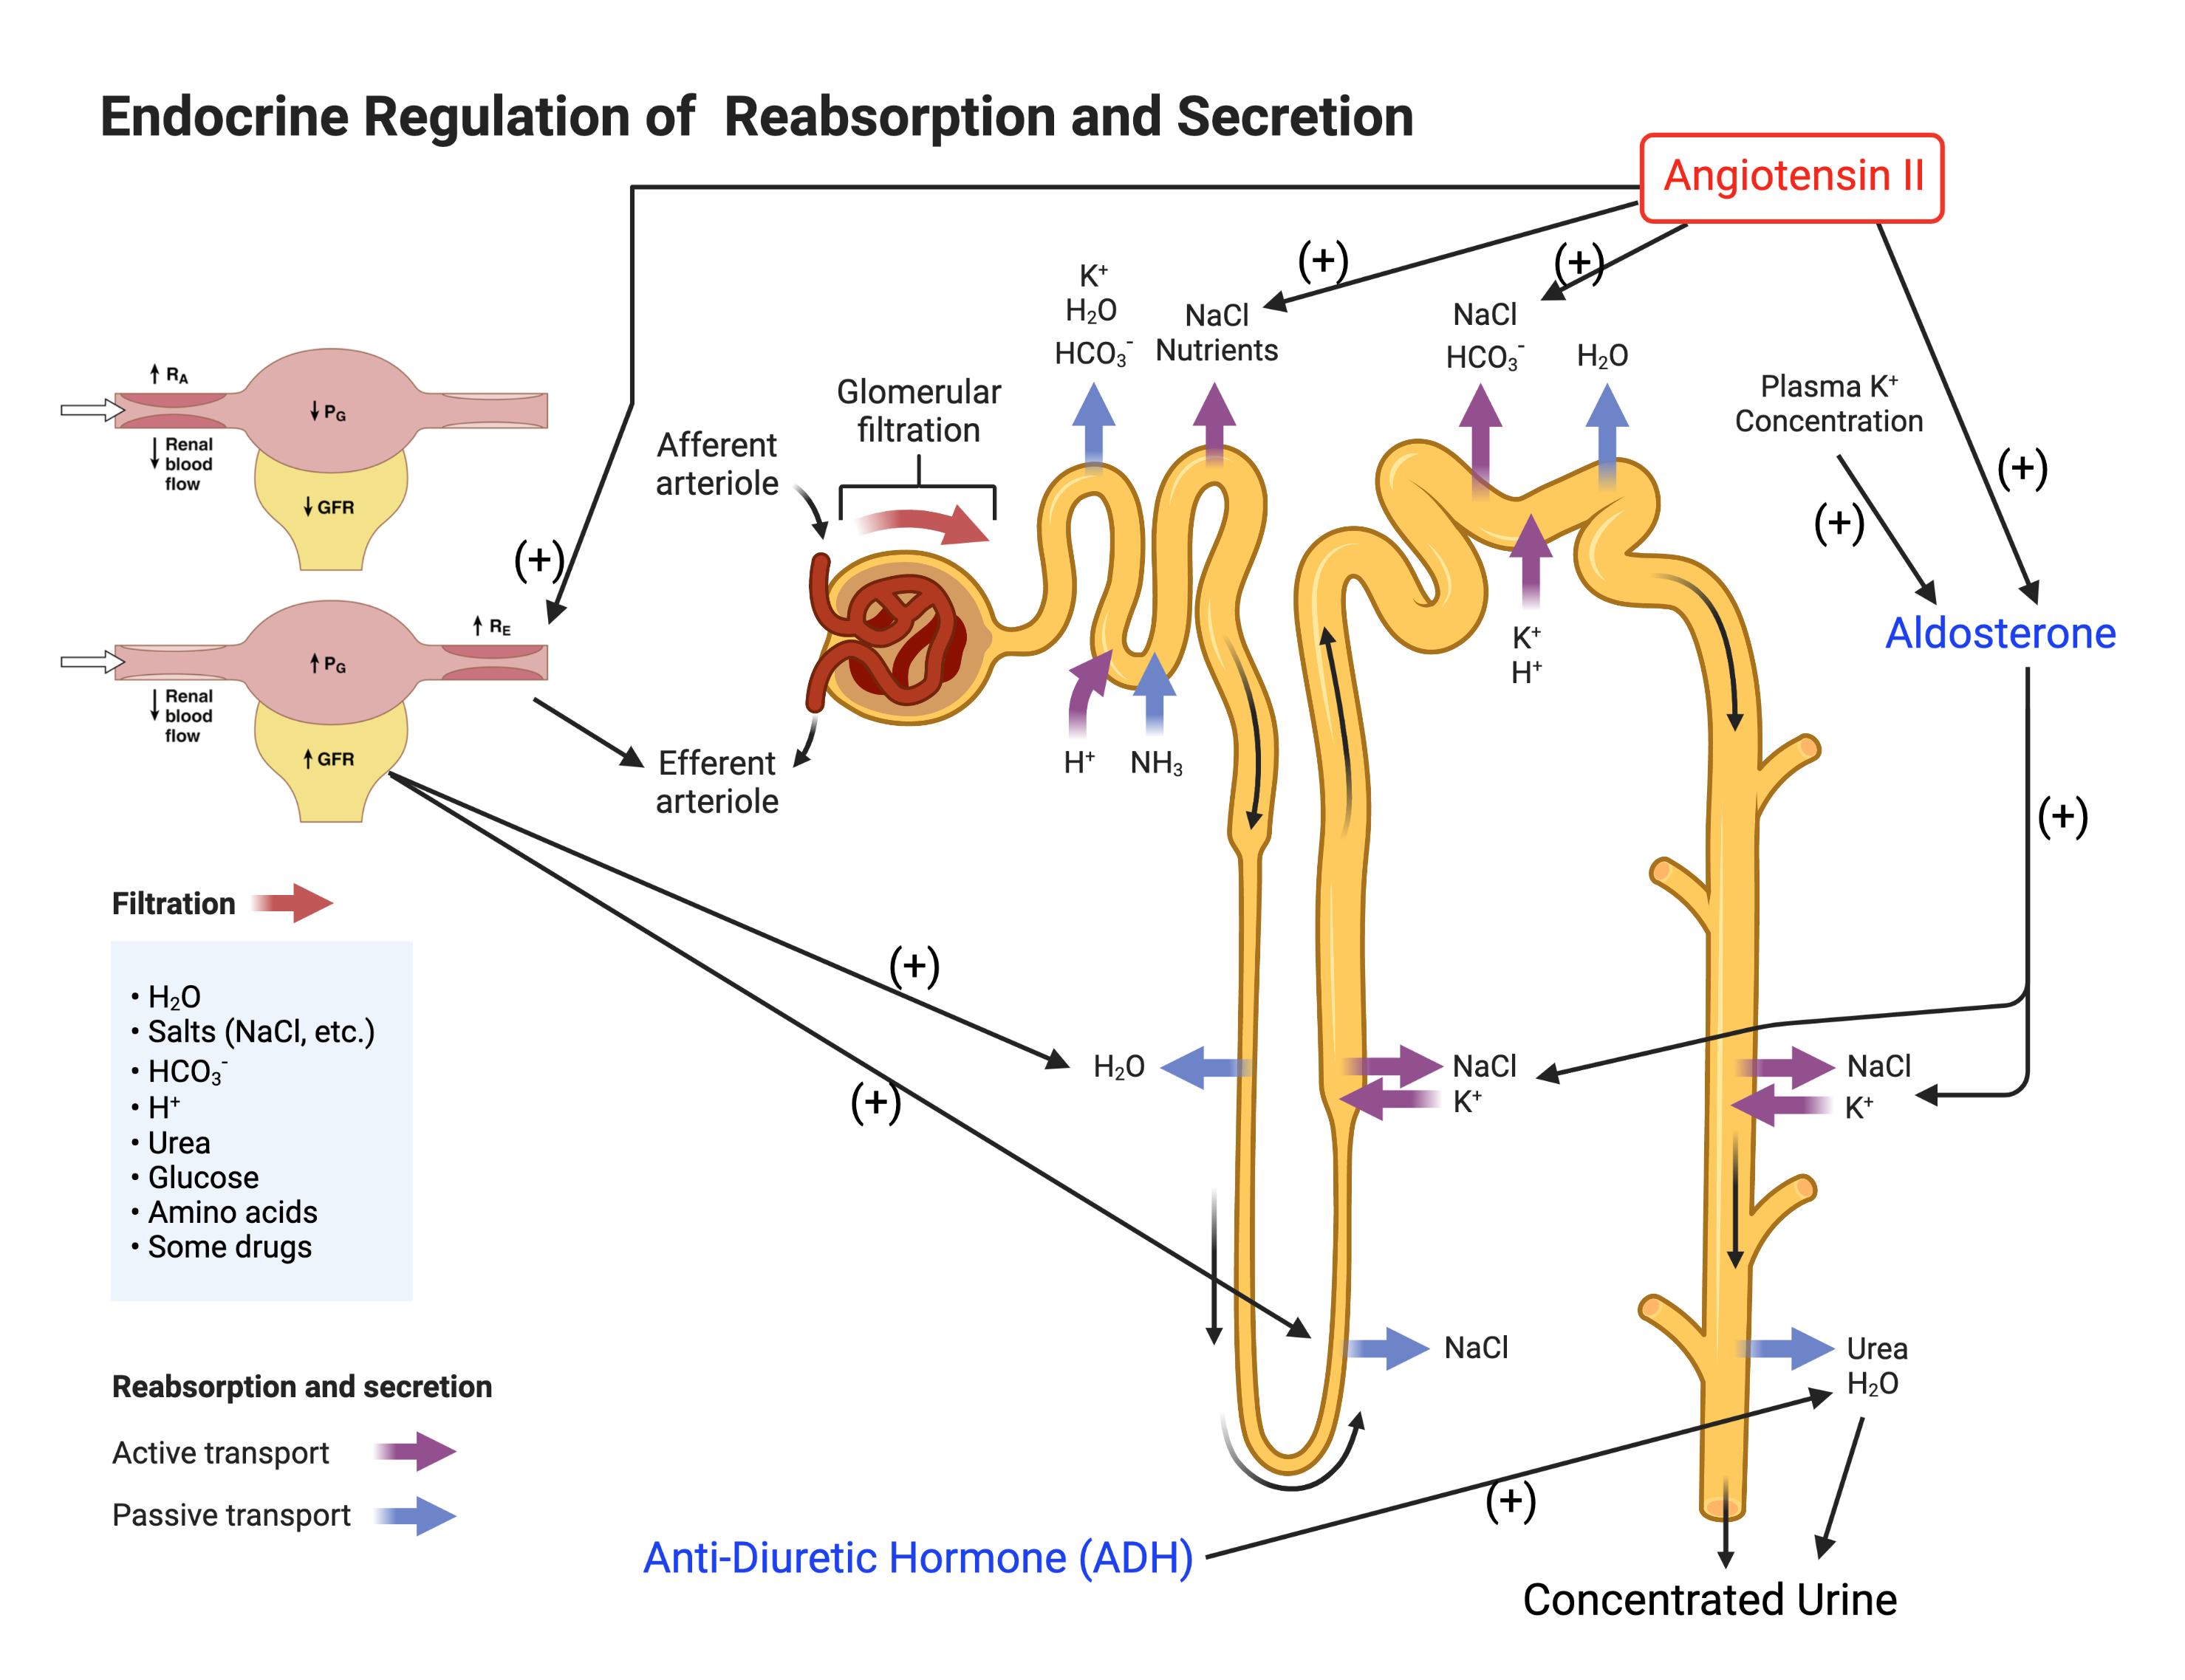
\includegraphics[width=1\linewidth]{./figure/Endocrine_Regulation.png}
    \caption{Integrated Action of Hormones \footnotesize{(Created with BioRender.com)}}
    \label{fig:Endocrine_Regulation}
\end{figure}

\subsubsection{Water Balance}

The intentional and incidental loss of water requires regular ingestion and absorption of water. Situations with more water loss than intake is a negative water balance. Situations with more water intake than loss is a positive water balance.

\begin{equation}
    Water Balance = Water Intake - Water Loss
    \label{water_balance}
\end{equation}

Monitoring water balance occurs through the monitoring of plasma osmolarity by the anterior hypothalamus (osmoreceptors). The response to changes in osmolarity involves ADH which has multiple end organ effects, including those that influence perception (thirst) and behavior (drinking). 

\paragraph{Response to Negative Water Balance}

\begin{enumerate}
\item Water is continuously lost from the body in sweat and in water vapor from the mouth and nose, as well as in urine (the kidneys must continue making urine to for waste excretion). If water is not replaced by drinking water, then plasma osmolarity increases. 
\item Increased plasma osmolarity stimulates osmoreceptors in the anterior hypothalamus, which are stimulated by changes in osmolarity of less than 1 mOsm/L. Stimulation of the hypothalamic osmoreceptors has two effects. It stimulates thirst, which drives drinking behavior. It also stimulates secretion of ADH from the posterior pituitary gland. 
\item The posterior pituitary gland secretes ADH. ADH circulates in the blood to the kidneys, where it produces increased water reabsorption. As more water is reabsorbed urine osmolarity increases and urine volume decreases (concentrated urine). 
\item Increased water reabsorption means that more water is returned to the body fluids. Coupled with increased thirst and drinking behavior, plasma osmolarity is decreased.
\end{enumerate}

The overall response is an excellent example of coordinated homeostatic negative feedback.  The original disturbance (increased plasma osmolarity) causes a set of feedback responses (thirst, secretion of ADH and increased water reabsorption) that decrease plasma osmolarity \cite{hall_guyton_2020}. Negative water balance results in concentrated urine.

\paragraph{Response to Positive Water Balance}

\begin{enumerate}
\item  Ingested water is distributed throughout the body fluids. Because the amount of solute in the body is unchanged, the added water dilutes the body fluids and cause a decrease in plasma osmolarity. 
\item The decrease in plasma osmolarity inhibits osmoreceptors in the anterior hypothalamus. 
\item Inhibition of the osmoreceptors has two effects. It decreases thirst and suppresses water drinking behavior. It also inhibits secretion of ADH from the posterior pituitary gland. 
\item When ADH secretion is inhibited, circulating levels of ADH are reduced and less ADH is delivered to the kidneys. Lower ADH levels decreases water reabsorption and water is excreted, decreasing urine osmolarity and increasing urine volume (diluted urine). 
\item Because less water is reabsorbed, less water is returned to the circulation. Coupled with the inhibition of thirst and the suppression of water drinking, plasma osmolarity increases back toward the normal value.
\end{enumerate}

The overall response is an excellent example of coordinated homeostatic negative feedback.  The original disturbance (decreased plasma osmolarity) causes a set of feedback responses (decreased thirst, less secretion of ADH and decreased water reabsorption) that increase plasma osmolarity \cite{hall_guyton_2020}. Positive water balance results in diluted urine.

\paragraph{Electrolyte Induced Changes to Osmolarity}
Water balance is not the only change that alters osmolarity and trigger the osmoreceptor - ADH response. Changes to osmolarity due to changes in solute concentrations also trigger the osmoreceptor - ADH response. The response coordinated by ADH primarily changes water content to adjust osmolarity, but they also facilitate correction of solute concentrations (though not solute content). For example, if $Na^+$ content increases with no change in water then $Na^+$ concentration increases along with plasma osmolarity. This hypernatremia induced increase in osmolarity first causes a shift in water out of the ICF, which partially reduces but does not normalize the ECF osmolarity. The still higher than normal osmolarity activates osmoreceptors that result in the release of ADH. ADH results in thirst, increased intake of water, and reduced loss of water. Together this response dilutes the plasma so that $Na^+$ concentration is reduced along with osmolarity. A consequence is higher plasma volume and therefore higher blood volume, which may result in higher blood pressure. Ideally the kidneys continue to correct this problem with less $Na^+$ reabsorption that returns plasma volume to a normal range.

\subsubsection{Blood Pressure}

Blood volume influences blood pressure (BP). Short term regulation of BP was covered in Chapter \ref{chp:circulation} on Circulation, primarily via the baroreceptors (quick, neural responses to altered BP). The role of the kidneys in BP regulation is a slower responding, and longer acting, regulatory system.

\paragraph{Renin Angiotensin II - Aldosterone System (RAAS)}

The RAAS system (depicted in Figure \ref{fig:raas}) is initiated in the kidneys in response to reduced fluid volume that decreases BP, RBF and GFR. In response the kidneys produce and secrete the hormone renin. Renin activates angiotension I which will be converted to angiotension II by angiotensin converting enzyme (ACE). Angiotension II (which has already been discussed in the section on GFR) directly influences kidney function by promoting both $Na^+$ and water reabsorption. It also activates aldosterone and ADH and to promote water and $Na^+$ reabsorption, and decrease tubular secretion. Angiotension II also directly promotes vasoconstriction of vascular smooth muscle. The overall effect of these events is increased blood pressure through vascular tone and increased blood volume.

\begin{figure}[!h]
    \centering
    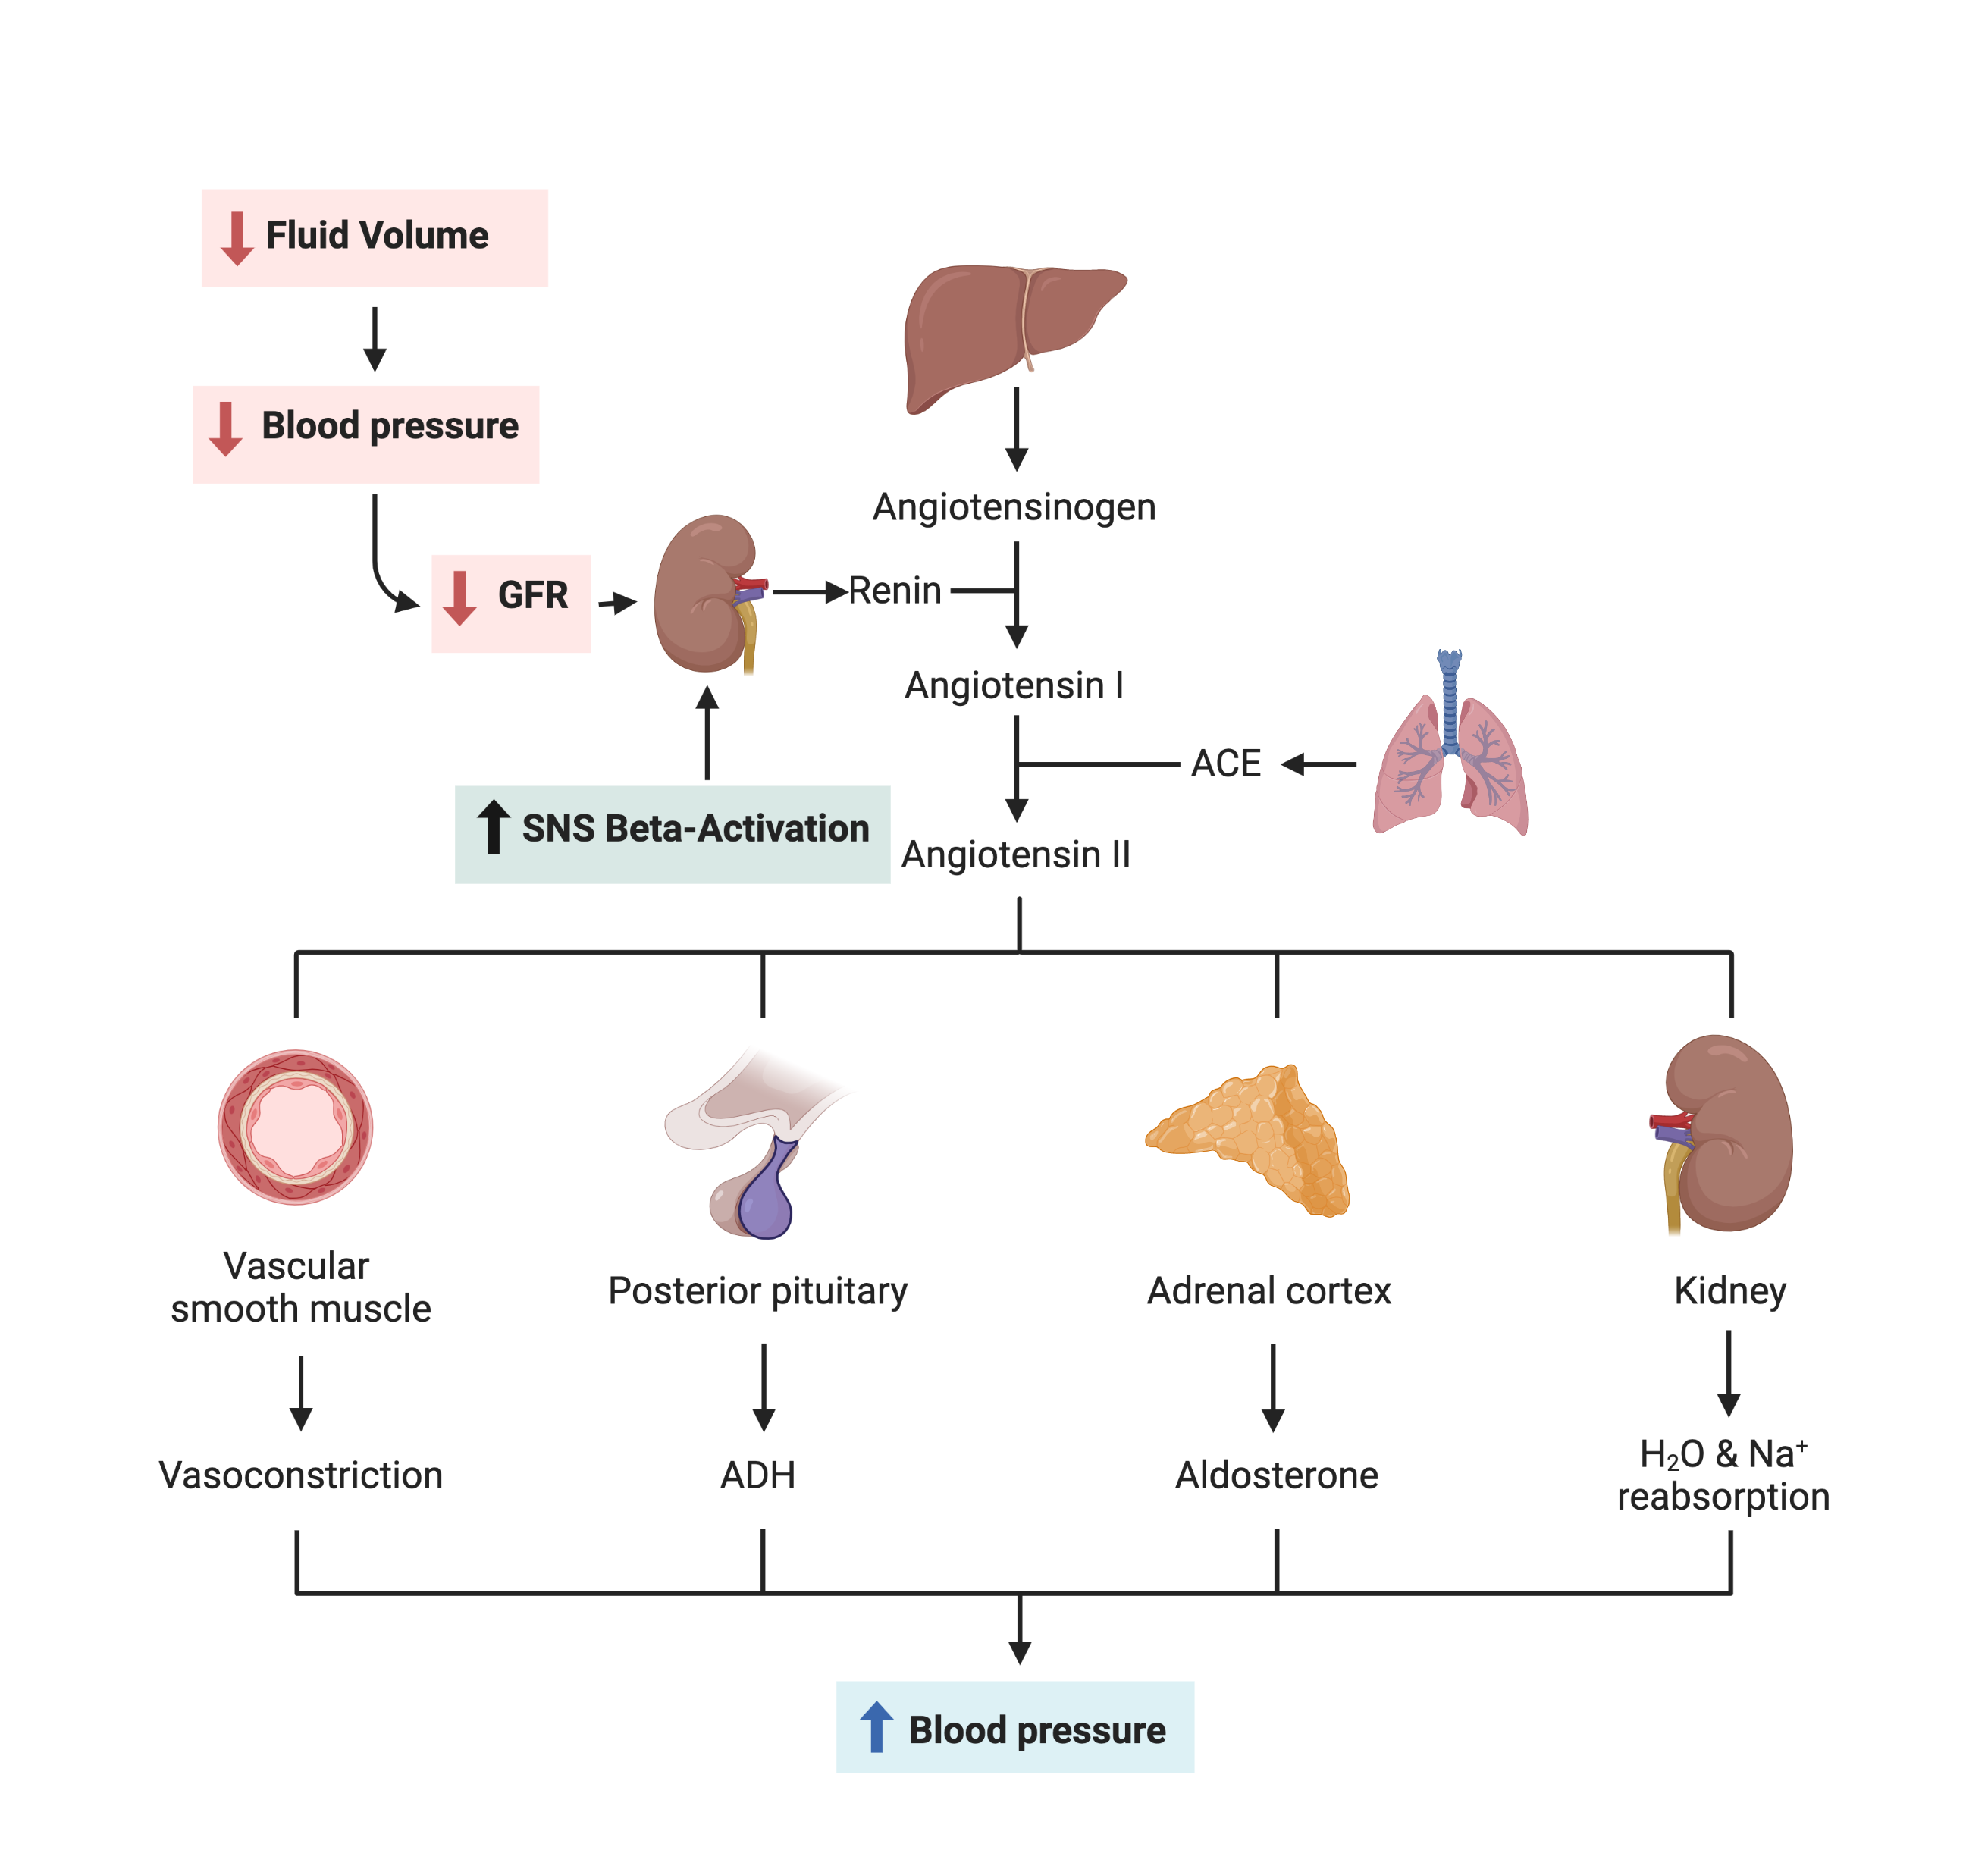
\includegraphics[width=1\linewidth]{./figure/raas.png}
    \caption{Renin Angiotensin System \footnotesize{(Created with BioRender.com)}}
    \label{fig:raas}
\end{figure}

\paragraph{RAAS Gone Wrong - Heart Failure \& ACE-Inhibition}

The events of RAAS depicted in Figure \ref{fig:raas} can go wrong. With chronic heart failure (HF) there can be reduced BP, or even with preserved BP but lower cardiac output, reduced RBF and GFR, that promotes the secretion of renin by the kidneys. In the context of HF, RAAS increases preload due to an increased vascular volume. The increased preload adds additional burden to an already failing heart. RAAS also increases afterload due to an increased blood pressure and systemic vasoconstriction. The increased afterload also adds additional burden to an already failing heart. The result tends to be a further reduction in cardiac output and GFR which promotes more renin secretion. This positive feedback loop is far from positive for the health of the individual with HF. In such situations the best course of action for restoring stability is a class of medication referred to a ACE-Inhibitors (ACE-I, i.e. captopril, lisinopril, enalapril) that block the enzyme at converts angiotension I to angiotensin II. ACE-I are also a preferred treatment for HTN (high blood pressure). Rather than forcing diuresis (as a diuretic does, which can create hypokalemia), they prevent anti-diuresis. Anti-anti diuresis is a gentle and physiologically stable approach to diuresis that prevents one of the several deleterious responses to reduced GFR due to HF. The therapuetic benefit of ACE-I goes beyond preventing anti-diuresis and includes reducing the release of aldosterone, and preventing angiotensin II from directly vasoconstricting blood vessels (increasing TPR and DBP), and directly resulting in water and $Na^+$ reabsorption.

\paragraph{Overall Integration of Renal Mechanisms and Arterial Pressure}

Figure \ref{fig:integrated_renal_bp} is a directed graph that depicts the closed loop integration of renal and circulatory systems through the renal regulation of blood volume, and the arterial pressure influence over renal excretion. 

\begin{figure}[!h]
    \centering
    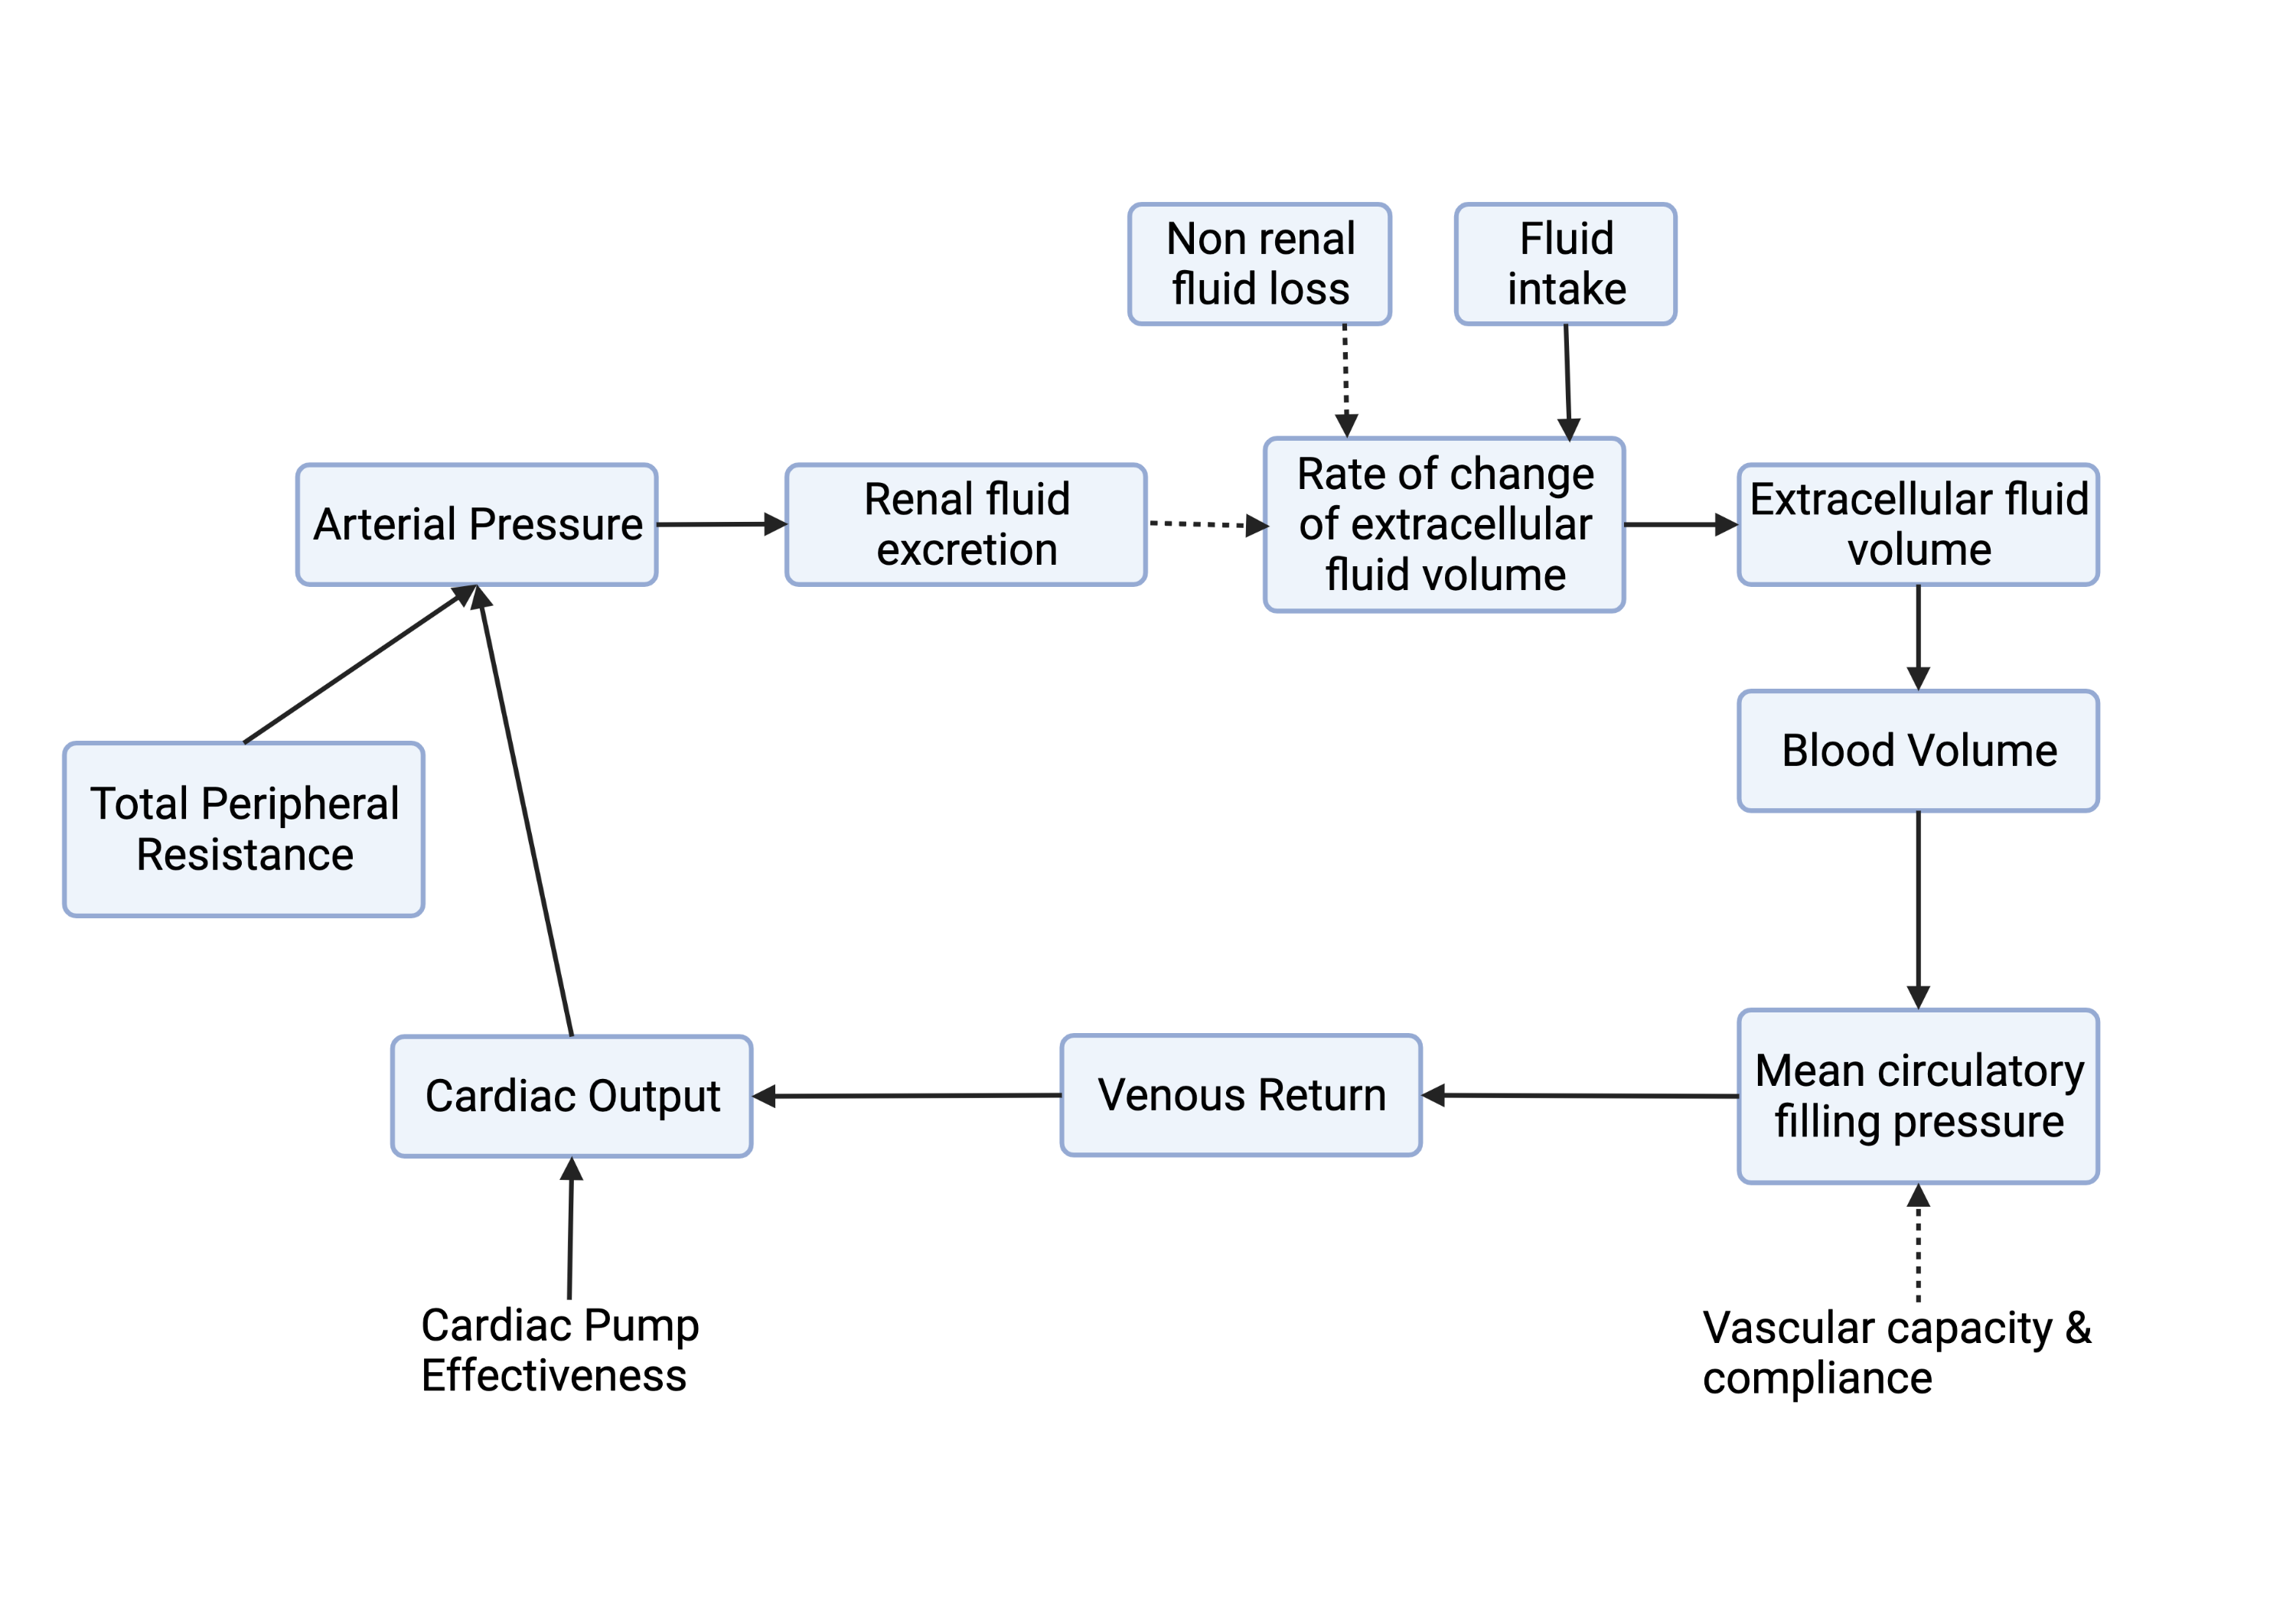
\includegraphics[width=1\linewidth]{./figure/integrated_renal_bp.png}
    \caption{Integration of Renal Mechanisms with Arterial Pressure  \footnotesize{(Modified from \cite{hall_guyton_2020} with BioRender.com)}}
    \label{fig:integrated_renal_bp}
\end{figure}

The variables in Figure \ref{fig:integrated_renal_bp} are familiar other than he mean circulatory filing pressure ($P_{mcf}$). $P_{mcf}$ is a variable created by Guyton in a model of renal blood pressure regulation \cite{rothe_mean_1993}. $P_{mcf}$ is defined as the mean vascular pressure that exists with a stop in cardiac output and distribution of blood until all pressures are the same throughout the system. It is related to the fullness of the circulatory system. A change in $P_{mcf}$ is a useful index of a change in overall venous smooth muscle tone if the blood volume is not changed. $P_{mcf}$ estimates the pressure in the small veins and venules, which contain most of the blood and account for most of the compliance. In total, $P_{mcf}$ provides an estimate of the pressure that determines the rate of flow returning to the heart, independent of cardiac output.

\section{Integrative Exercise: Disturbances in Osmolarity}

The purpose of this integrative exercise is for the reader to integrate previous understanding with a slowly expanding new understanding in the area of disturbances in osmolarity. It is not intended that readers would memorize the sequences below, but rather understand them and, if needed, recreate them from thinking through the processes involved from an understanding of the principles. The short descriptions below do not include all of the possible trajectories or all of the physiological responses. With the next chapters on Respiration and Ventilation, one goal is to start considering the impact of ECF volume on hematocrit, and the fact that the volume of a RBC is intracellular.

Osmolarity is the concentration of osmotically active particles, expressed as milliosmoles per liter ($mOsm/L$). The normal value for osmolarity of the body fluids is approximately 290 $mOsm/L$ in both ECF and ICF since water will shift between these spaces until osmolarity equilibrates \cite{costanzo_physiology_2013}.

Plasma osmolarity ($mOsm/L$) can be estimated from the plasma $Na^+$ concentration ($mmol/L$), plasma glucose concentration ($mg/dL$), and blood urea nitrogen (BUN) ($mg/dL$), as these are the major solutes of ECF and plasma. 

\begin{equation}
Plasma Osmolarity = 2 \times [Na^+] + \frac{[Glucose]}{18} +\frac{[BUN]}{2.8}
\label{osmolarity}
\end{equation}
\paragraph{}
The $Na^+$ concentration is multiplied by 2 because $Na^+$ is balanced by an equal concentration of negative ions (in plasma, these anions are $Cl^-$ and $HCO_3^-$.)\footnotemark\footnotetext{Despite common assumptions that the outside of the cell is positive and the inside of the cell is negative, there is electroneutrality in both ECF and ICF fluid. Recall from Chapter \ref{chp:excitation} that membrane potentials are generated from the movement of the ions, not the concentration of the ions.} The glucose concentration in mg/dL is converted to mOsm/L when it is divided by 18. The BUN in mg/dL is converted to mOsm/L when it is divided by 2.8. Calculating Equation \ref{osmolarity} with the values of 140 $mmol/L$ of $Na^+$, 80 $mg/dL$ of glucose, and 15 $mg/dL$ for BUN results in 289.79 $mOsm/L$.

In the following sections volume contraction means a decrease in ECF volume. Volume expansion means an increase in ECF volume. In place of the more general terms isotonic, hypertonic and hypotonic the more specific terms isosmotic, hyperosmotic, and hyposmotic refer to the osmolarity of the ECF for the osmolarity disturbances. Consistent with Chapter \ref{chp:ecf_microcirculation}, an isosmotic disturbance means that there is no change in ECF osmolarity; a hyperosmotic disturbance means that there has been an increase in ECF osmolarity; and a hyposmotic disturbance means that there has been a decrease in ECF osmolarity.

\paragraph{Three-Step Approach}
To understand these disturbances, a three-step approach is recommended (\cite{costanzo_physiology_2013}):

\begin{enumerate}
\item Identify any change occurring in the ECF (e.g., Was solute added to the ECF? Was water lost from the ECF?).
\item Decide whether that change will produce an increase, a decrease, or no change in ECF osmolarity. 
\item If there is a change in ECF osmolarity, determine whether water will shift into or out of the cells to reestablish equality between ECF osmolarity and ICF osmolarity. If there is no change in ECF osmolarity, no water shift will occur. If there is a change in ECF osmolarity, then a water shift must occur. 
\end{enumerate}

\subsection{Isosmotic Volume Contraction: Diarrhea}

Diarrhea results in a lose a large volume of fluid from the gastrointestinal tract. The osmolarity of the fluid lost is approximately equal to that of the ECF (isosmotic).  ECF volume decreases, but there is no accompanying change in ECF osmolarity. Therefore there is no need for a fluid shift across cell membranes and ICF volume remains unchanged. In the new steady state, ECF volume decreases and the osmolarities of ECF and ICF are unchanged. The decrease in ECF volume means that blood volume (a component of ECF) also is reduced, which produces a decrease in arterial pressure. Other consequences of diarrhea include increased hematocrit and increased plasma protein concentration. The

\subsection{Hyperosmotic Volume Contraction: Sweating}

Water deprivation (negative mass balance of water) in situations with sweating (hot environments and/or high metabolism) results in net loses to both NaCl and water in sweat. Sweat is hyposmotic relative to ECF. Sweat contains relatively more water than solute. When sweating hyposmotic fluid is lost from the ECF. ECF volume decreases and ECF osmolarity increases. ECF osmolarity is transiently higher than ICF osmolarity, and this difference in osmolarity causes water to shift from ICF into ECF until ICF and ECF osmolarity  equalizes. In the new steady state, both ECF and ICF volumes are decreased and ECF and ICF osmolarities increased. In hyperosmotic volume contraction, the plasma protein concentration is increased but the HcT is unchanged. The explanation for the increase in plasma protein concentration is straightforward: Fluid is lost from ECF, and the plasma protein remaining behind becomes concentrated. It is less obvious, however, why the hematocrit is unchanged. Loss of fluid from ECF alone would cause an increase in the concentration of red blood cells and an increase in HcT. However, there also is a fluid shift in this disturbance: Water moves from ICF to ECF. Because RBCs are cells, water shifts out of them, decreasing their volume. Thus, the concentration of red blood cells increases, but red blood cell volume decreases. The two effects offset each other, and HcT is unchanged. The shift of water from ICF to ECF offsets the loss of ECF from water loss.

\subsection{Hyposmotic Volume Contraction: Adrenal Insufficiency}

Adrenal insufficiency includes a deficiency in aldosterone, a hormone that promotes $Na^+$ reabsorption. Aldosterone deficiency results in excess NaCl excreted in the urine. Because NaCl is an ECF solute, ECF osmolarity decreases. ECF osmolarity is less than ICF osmolarity and causes water to shift from ECF to ICF until osmolarity equilibrium. In the new steady state, both ECF and ICF osmolarities are lower than normal. The shift of water results in decreased ECF volume and increased ICF volume. In hyposmotic volume contraction, both plasma protein concentration and HcT will be increased because of the decrease in ECF volume. HcT also increases because of the shift of water into red blood cells, increasing cell volume. 

\subsection{Isosmotic Volume Expansion: Infusion of NaCl} 

An infusion of isotonic NaCl presents the opposite clinical picture of losing isotonic fluid through diarrhea. Because NaCl is an extracellular solute, all isotonic NaCl solution is added to the ECF, causing an increase in ECF volume but no change in ECF osmolarity. There is no shift of water between ICF and ECF because there is no difference in osmolarity between the two compartments. Both plasma protein concentration and HcT decrease (i.e., be diluted) because of the increase in ECF volume. 

\subsection{Hyperosmotic Volume Expansion: High NaCl Intake} 

Ingesting dry NaCl (for example, eating a salty snack) increases the total amount of $Na^+$ in the ECF and osmolarity increases transiently as the higher ECF osmolarity causes water to shift from ICF to ECF, decreasing ICF volume and increasing ECF volume. In the new steady state, both ECF and ICF osmolarities are higher than normal and equal to each other. Because of the shift of water out of cells, ICF volume will decrease and ECF volume will increase. In hyperosmotic volume expansion, both plasma protein concentration and hematocrit will decrease due to the increase in ECF volume. Hematocrit also will be decreased because of the water shift out of the red blood cells. 

\subsection{Hyposmotic Volume Expansion: SIADH} 

Syndrome of inappropriate antidiuretic hormone (SIADH) secretes inappropriately high levels of ADH, which promotes too much water reabsorption. The excess water is retained and distributed throughout the total body water. ECF is diluted and transiently has a lower osmolarity. Water shifts into the ICF since it has higher osmolarity. When compared with the normal state, ECF and ICF volumes are both increased and ECF and ICF osmolarities will be decreased. In hyposmotic volume expansion, plasma protein concentration is decreased by dilution. The hematocrit is unchanged as a result of two offsetting effects: The concentration of red blood cells decreases because of dilution, but RBC volume increases because water shifts into the cells. But this increase in RBC volume (due to water) does not necessarily increase oxygen carrying capacity of HbG so maintaining HcT in the situation of hyposmotic volume expansion does not necessarily mean oxygen carrying capacity is normal.



\section{\textit{Muscle Connections}}

\subsection{Speculation on Water Homeostasis in Muscle Function \& Frailty}
Older adults have reduced thirst sensation and the ability to concentrate urine, together this results in increased ECF osmolarity (hyperosmotic stress) \cite{lorenzo_role_2019}. Hyperosmotic stress leads to cell dehydration (reduced ICF), which has consequences for the intracellular protein structure and function. In severe situations this can result in cell damage. There is also some evidence to suggest that cell volume may act as a signal, with cell swelling acting as an anabolic signal (promotes hypertrophy) and cell shrinkage acting as a catabolic signal (promotes atrophy). One possible reason, or contributing factor, for the age related progressive loss in muscle mass and strength may be impaired ECF - ICF water homeostasis that originates from mild kidney insufficiency and a loss of thirst. Intracellular water content in lean mass has been related to muscle strength, functional capacity, and frailty risk, and has been proposed as an indicator of muscle quality and cell hydration \cite{lorenzo_role_2019}. Muscle weakness can promote further decreases in fluid (and nutrient) intake due to challenges in ADLs. This can occur directly with difficulty attaining the necessary muscle tension for performing ADLs (either basic ADLs or instrumental ADLs), or with the accumulation of objective fatigue (difficulty sustaining ADLs)\cite{collins_heart_2015}.  Several chronic conditions that include renal insufficiency such as diabetes, high blood pressure, chronic heart failure, obstructive pulmonary disease and (obviously) renal failure all share a common feature of muscle catabolism, atrophy and weakness. With these conditions the atrophy and weakness seem to go beyond disuse atrophy \cite{adams_skeletal_2006}. A common, and plausible, feature of these conditions may be water homeostasis. 


\subsection{Rhabdomyolosis}
Rhabdomyolosis is a condition in which damaged skeletal muscle breaks down rapidly. Symptoms include muscle pain; signs include weakness, muscle stiffness and edema. Signs may also include tea-colored urine, an irregular heartbeat, vomiting, and confusion. A positive urine myoglobin test provides supportive evidence. Myoglobin is harmful to nephrons so if rhabdomyolysis is severe it may lead to kidney failure. Common causes of muscle damage include crush injury, strenuous exercise, medications (including statins for lowering blood cholesterol), or substance abuse. Less common causes include infections, electrical injury, heat stroke, prolonged immobilization, lack of blood flow to a limb, or snake bites.

\subsection{Uromysotisis Poisoning}

A fictional condition created by Jerry Seinfeld and Larry David to justify Jerry's need to urinate in a mall parking garage when he and his friends lost their car and had to wander the garage for hours (See \href{https://www.youtube.com/watch?v=OG6b7KJ1Ah0}{Seinfeld-Parking Garage}). According the Jerry Seinfeld and Larry David uromysotisis poisoning is a potentially deadly condition resulting from holding in one's urine for a prolonged period of time. The condition can result in acute poisoning when one is restricted by the arbitrary rules of society. Common treatments for uromysotisis include the "pee party".

\section{Summary}
Mass balance is an essential concept for physical therapy practice. The need for intake and the intentional or incidental output is central to physiology and wellness. The need for intake frames our activities of daily living. Having the mass balance to sustain an environment for muscle function (ECF) requires muscles to function (performing activities). Renal function, including clearance, filtration, reabsorption, secretion and excretion are essential to mass balance. Kidneys ensure not only that waste products are eliminated but that extra micronutrients (or even nutrients in extreme cases) are eliminated; or that when there are not extra micronutrients that their elimination is reduced. It is much easier to ensure mass "balance" by adjusting what we eliminate than by adjusting what is ingested. The kidneys allow that freedom. In doing this primary role that kidneys influence, and regulate, blood volume and therefore blood pressure. In turn, the kidneys are regulated based on blood volume and blood pressure. There is an exquisite set of integrated renal, blood pressure and hormonal responses that keeps fluid volume, blood volume, blood osmolarity, blood pressure and micronutrient content and concentration balanced. With aging or certain chronic conditions the physiological range of integrated renal regulation may be reduced and behavior must change to allow for easier regulation (i.e., regulating water and $Na^+$ intake through diet makes it easier for the kidneys to regulate water and $Na^+$ levels by varying water and $Na^+$ output).

\subsection{Next Step}

With a deeper understanding of mass balance we can now proceed to the mass balance of oxygen and carbon dioxide in the next two chapters. Chapter \ref{chp:blood_oxygen} on Respiration focuses on gas exchange between the alveoli and blood. Chapter \ref{chp:alveolar_oxygen} on Ventilation focuses on air exchange between the environment and the alveoli (breathing).



\printbibliography[heading=subbibintoc]